% Created 2019-08-13 Tue 12:50
\documentclass[12pt,twoside]{article}
\usepackage[utf8]{inputenc}
\usepackage[T1]{fontenc}
\usepackage{fixltx2e}
\usepackage{graphicx}
\usepackage{grffile}
\usepackage{longtable}
\usepackage{wrapfig}
\usepackage{rotating}
\usepackage[normalem]{ulem}
\usepackage{amsmath}
\usepackage{textcomp}
\usepackage{amssymb}
\usepackage{capt-of}
\usepackage{hyperref}
\usepackage{lscape}
\usepackage{fancyhdr}
\usepackage{multirow}
\usepackage{multicol}
\author{David Balchen}
\date{\today}
\title{The Usage Bible}
\hypersetup{
 pdfauthor={David Balchen},
 pdftitle={The Usage Bible},
 pdfkeywords={},
 pdfsubject={},
 pdfcreator={Emacs 24.5.1 (Org mode 8.3.4)}, 
 pdflang={English}}
\begin{document}

\maketitle
\pagenumbering{gobble}
\includegraphics[width=16cm]{Pictures/Andrejevi1.jpg}
\newpage 
\includegraphics[width=13cm]{Pictures/postal5.png}
%\addtolength{\oddsidemargin}{-.25in}
\addtolength{\oddsidemargin}{0in}
\addtolength{\evensidemargin}{-01.25in}
\addtolength{\textwidth}{1.4in}
\addtolength{\topmargin}{-1.25in}
\addtolength{\textheight}{2.45in}
\setcounter{tocdepth}{3}
\vspace*{1cm} 
\newpage
\pagenumbering{roman}
\setcounter{tocdepth}{2}
\pagestyle{fancy}
\fancyhf[ROF,LEF]{\bf\thepage}
\fancyhf[C]{}
\setcounter{tocdepth}{2}
\tableofcontents
 \newpage
\pagenumbering{arabic}
\section{Usage Overview}
\label{sec:orgheadline8}
Usage is a broad term used to refer to network event records that are used for rating and charging our customers. In telephony we tend to think of usage
in two ways, \textbf{Voice} or \textbf{Data}.\\
\subsection{Usage Record Formats}
\label{sec:orgheadline1}
Usage records come from the switch in a verity of formats depending on the equipment used.
\mbox{} \\
\mbox{} \\
\textbf{Voice}\\
   Voice usage can come in one of two formats:
\begin{enumerate}
\item \textbf{Alcatel Lucent (APLX)} - The \textbf{Alcatel Lucent APLX} switch record
are found mostly in the Maine market.
\item \textbf{Nortel (NTI)} - The \textbf{NORTEL NTI} switch record is the most common
voice record format.
\item \textbf{CIBER} - For \emph{InCollect and OutCollect} processing.
\end{enumerate}
\mbox{} \\
\textbf{Data}\\
   For data there is a format for each type:
\begin{enumerate}
\item \textbf{SMSC} - The \textbf{SMS} record type comes in the \textbf{Motorola} format.
\item \textbf{AAA Server} - 
\begin{itemize}
\item \textbf{PGW} - P-Gateway \textbf{LTE} data usage
\item \textbf{ECS} - ECS \textbf{3G and lower} data usage.
\item \textbf{AAA} - Raw AAA usage found on the CallDump only.
\item \textbf{TAS} - \emph{Volte} Voice over \textbf{LTE}.
\end{itemize}
\item \textbf{VALI} - \emph{Premium SMS (Valista)} pre-rated records.
\item \textbf{GSM Roaming} - Voice and data records from our customers who are
roaming in Europe and other \textbf{GSM} countries.
\item \textbf{MMSC} - Used for both pictures and picture messaging text only
(treated as an \textbf{SMS} message in the system).
\item \textbf{TAP} - Used for \textbf{Incollect/Outcollect 4G} processing.
\end{enumerate}
\newpage
\subsection{Network Elements}
\label{sec:orgheadline2}
The list below is the name of \textbf{switches/network elements} that produce usage and where that usage is stored in \textbf{TOPS}.
Except for the \textbf{TAP} files, all are readable as either \textbf{CIBER} of \textbf{UFF}.
\mbox{} \\
\footnotesize

\begin{longtable}{l|l|l}
\hline
\textbf{Element} & \textbf{New Host} & \textbf{New Directory}\\
\hline
\endfirsthead
\multicolumn{3}{l}{Continued from previous page} \\
\hline

\textbf{Element} & \textbf{New Host} & \textbf{New Directory} \\

\hline
\endhead
\hline\multicolumn{3}{r}{Continued on next page} \\
\endfoot
\endlastfoot
\hline
APPL & kpr01bchl2 & /pkgbl02/inf/prdsys/prodwrk2/var/usc/projs/up/physical/NTI1/APPL\\
ASHE & kpr01bchl2 & /pkgbl02/inf/prdsys/prodwrk2/var/usc/projs/up/physical/NTI1/ASHE\\
CDP & kpr01bchl2 & /pkgbl02/inf/prdsys/prodwrk2/var/usc/projs/up/physical/CONT/CDP\\
CDR2 & kpr01bchl2 & /pkgbl02/inf/prdsys/prodwrk2/var/usc/projs/up/physical/NTI1/CDR2\\
CIB\_IC & kpr01bchl2 & /pkgbl02/inf/prdsys/prodwrk2/var/usc/projs/up/physical/switch/DIRI\\
CIB\_OCR & kpr01bchl2 & /pkgbl02/inf/prdsys/prodwrk2/var/usc/projs/up/physical/switch/SYNR\\
CLIN & kpr01bchl2 & /pkgbl02/inf/prdsys/prodwrk2/var/usc/projs/up/physical/NTI1/CLIN\\
COLU & kpr01bchl2 & /pkgbl02/inf/prdsys/prodwrk2/var/usc/projs/up/physical/NTI1/COLU\\
CONG & kpr01bchl2 & /pkgbl02/inf/prdsys/prodwrk2/var/usc/projs/up/physical/NTI1/CONG\\
ECS & kpr01bchl2 & /pkgbl02/inf/prdsys/prodwrk2/var/usc/projs/up/physical/AAA/AAA1\\
EURE & kpr01bchl2 & /pkgbl02/inf/prdsys/prodwrk2/var/usc/projs/up/physical/NTI1/EURE\\
GRAN & kpr01bchl2 & /pkgbl02/inf/prdsys/prodwrk2/var/usc/projs/up/physical/NTI1/GRAN\\
GREE & kpr01bchl2 & /pkgbl02/inf/prdsys/prodwrk2/var/usc/projs/up/physical/NTI1/GREE\\
GSM\_IR & kpr01bchl2 & /pkgbl02/inf/prdsys/prodwrk2/var/usc/projs/up/physical/GSMI/GSMS\\
GSM\_IR & kpr01bchl2 & /pkgbl02/inf/prdsys/prodwrk2/var/usc/projs/up/physical/GSMI/GSMV\\
JOHN & kpr01bchl2 & /pkgbl02/inf/prdsys/prodwrk2/var/usc/projs/up/physical/NTI1/JOHN\\
JOPL & kpr01bchl2 & /pkgbl02/inf/prdsys/prodwrk2/var/usc/projs/up/physical/NTI1/JOPL\\
KNOX & kpr01bchl2 & /pkgbl02/inf/prdsys/prodwrk2/var/usc/projs/up/physical/NTI1/KNOX\\
LLYN & kpr01bchl2 & /pkgbl02/inf/prdsys/prodwrk2/var/usc/projs/up/physical/APLX/LLYN\\
LROE & kpr01bchl2 & /pkgbl02/inf/prdsys/prodwrk2/var/usc/projs/up/physical/APLX/LROE\\
LTE & kpr01bchl2 & /pkgbl02/inf/prdsys/prodwrk2/var/usc/projs/up/physical/PGW/PGW1\\
LTE & kpr01bchl2 & /pkgbl02/inf/prdsys/prodwrk2/var/usc/projs/up/physical/GSMI/GSMD\\
MADI & kpr01bchl2 & /pkgbl02/inf/prdsys/prodwrk2/var/usc/projs/up/physical/NTI1/MADI\\
MEDF & kpr01bchl2 & /pkgbl02/inf/prdsys/prodwrk2/var/usc/projs/up/physical/NTI2/MEDF\\
MMSC & kpr01bchl2 & /pkgbl02/inf/prdsys/prodwrk2/var/usc/projs/up/physical/SMS\_MMS/PMG1\\
MMSC & kpr01bchl2 & /pkgbl02/inf/prdsys/prodwrk2/var/usc/projs/up/physical/SMS\_MMS/PTX1\\
MORG & kpr01bchl2 & /pkgbl02/inf/prdsys/prodwrk2/var/usc/projs/up/physical/APLX/MORG\\
NEWB & kpr01bchl2 & /pkgbl02/inf/prdsys/prodwrk2/var/usc/projs/up/physical/NTI2/NEWB\\
OKLA & kpr01bchl2 & /pkgbl02/inf/prdsys/prodwrk2/var/usc/projs/up/physical/NTI2/OKLA\\
OMAH & kpr01bchl2 & /pkgbl02/inf/prdsys/prodwrk2/var/usc/projs/up/physical/NTI1/OMAH\\
OWAS & kpr01bchl2 & /pkgbl02/inf/prdsys/prodwrk2/var/usc/projs/up/physical/NTI2/OWAS\\
PEO2 & kpr01bchl2 & /pkgbl02/inf/prdsys/prodwrk2/var/usc/projs/up/physical/NTI2/PEO2\\
ROC2 & kpr01bchl2 & /pkgbl02/inf/prdsys/prodwrk2/var/usc/projs/up/physical/NTI2/ROC2\\
SALI & kpr01bchl2 & /pkgbl02/inf/prdsys/prodwrk2/var/usc/projs/up/physical/NTI2/SALI\\
SMS\_NSN & kpr01bchl2 & /pkgbl02/inf/prdsys/prodwrk2/var/usc/projs/up/physical/SMS\_MMS/MOT\\
SMS\_NSN & kpr01bchl2 & /pkgbl02/inf/prdsys/prodwrk2/var/usc/projs/up/physical/GSMI/GSMT\\
TAS & kpr01bchl2 & /pkgbl02/inf/prdsys/prodwrk2/var/usc/projs/up/physical/TAS/TAS1\\
VALISTA & kpr01bchl2 & /pkgbl02/inf/prdsys/prodwrk2/var/usc/projs/up/physical/CONT/VALI\\
YAKI & kpr01bchl2 & /pkgbl02/inf/prdsys/prodwrk2/var/usc/projs/up/physical/NTI2/YAKI\\
TAP\_IN & kpr01bchl4 & /pkgbl04/inf/prdsys/prodwrk4/var/usc/projs/smm/DATA/TAPIN\\
TAP\_OUT & kpr01bchl4 & /pkgbl04/inf/prdsys/prodwrk4/var/usc/projs/smm/DATA/TAPOUT\\
APRM & kpr01bchl2 & /pkgbl02/inf/prdsys/prodwrk2/var/usc/projs/up/physical/switch/DATAIN\\
CIB\_IC & kpr01bchl2 & /pkgbl02/inf/prdsys/prodwrk2/var/usc/projs/up/physical/switch/DATACBR\\
CIB\_IC & kpr01bchl2 & /pkgbl02/inf/prdsys/prodwrk2/var/usc/projs/up/physical/switch/DIRI\\
CIB\_ICR & kpr01bchl2 & /pkgbl02/inf/prdsys/prodwrk2/var/usc/projs/apr/interfaces/output\\
SGW/DISP & kpr01bchl3 & /pkgbl03/inf/prdsys/operaprm/var/usc/LSN/input2\\
GSM\_IR & kpr01bchl4 & /pkgbl04/inf/prdsys/prodwrk4/var/usc/projs/smm/DATA/TAPIN\\
RAP\_IN & kpr01bchl4 & /pkgbl04/inf/prdsys/prodwrk4/var/usc/projs/smm/DATA/RAPIN\\
RAP\_OUT & kpr01bchl4 & /pkgbl04/inf/prdsys/prodwrk4/var/usc/projs/smm/DATA/RAPOUT\\
\hline
\end{longtable}

\normalsize
\newpage
\subsection{Pre-Pay and Data Roaming}
\label{sec:orgheadline3}

In addition to \textbf{Post-Pay} we also handle \textbf{Pre-Pay} which follows a
different flow using the diameter interface. The \textbf{Diameter
interface} is described as follows:

\begin{itemize}
\item \textbf{Diameter} is a \textbf{AAA} protocol, a type of computer networking
protocol for authentication, authorization and accounting \textbf{(AAA)}. 
\textbf{Diameter} controls communication
between the authenticator (Secure Ticket Authority, STA) and
any network entity requesting authentication. \textbf{Diameter Applications} 
extend the base protocol by adding new commands
and/or attributes, such as those for use of the Extensible
Authentication Protocol (\textbf{EAP}).
\end{itemize}
\subsection{Carrier Code and Names}
\label{sec:orgheadline4}
SQL Statement which produced this data:
\begin{verbatim}
select distinct carr_name, carr_cd from prm_app.PRM_REP_CARR_INFO
\end{verbatim}
\footnotesize

\begin{longtable}{l|l}
\hline
CARRIER\_NAME & CARRIER\_CODE\\
\hline
\endfirsthead
\multicolumn{2}{l}{Continued from previous page} \\
\hline

CARRIER\_NAME & CARRIER\_CODE \\

\hline
\endhead
\hline\multicolumn{2}{r}{Continued on next page} \\
\endfoot
\endlastfoot
\hline
AT\&T Mobility (USAAT) & USAAT\\
AT\&T Mobility (USACG) & USACG\\
AT\&T Mobility (USABS) & USABS\\
Pioneer Cellular (USAPI) & USAPI\\
T-Mobile (USATM) & USATM\\
Nex-Tech Wireless (USA6G) & USA6G\\
AT\&T Mobility (USAPB) & USAPB\\
AT\&T Mobility (USAMF) & USAMF\\
Sprint (USASG) & USASG\\
T-Mobile (USAW6) & USAW6\\
Sprint (USASP) & USASP\\
Verizon (USAVZ) & USAVZ\\
Vodafone Netherlands (NLDLT) & NLDLT\\
AT\&T Mobility (USACC) & USACC\\
\hline
\end{longtable}
\normalsize
\subsection{Usage Time Zones}
\label{sec:orgheadline5}
\begin{center}
\begin{tabular}{ll}
\hline
\textbf{Usage Type} & \textbf{TimeZone}\\
\hline
AAA & GMT\\
PGW/LTE & GMT\\
PMG/PTX & GMT\\
TAS & GMT\\
MOT/ALU & EST\\
VoLTE & Switch Location\\
Voice & Switch Location\\
CIBER & Switch Location\\
GSMD/V/S & GMT\\
\hline
\end{tabular}
\end{center}
\newpage
\subsection{Duplicate Record Keys}
\label{sec:orgheadline6}
Columns used to detect if a record is a duplicate.
\small
\begin{center}
\begin{tabular}{lll}
\hline
\textbf{MMS} & \textbf{SMS} & \textbf{Content}\\
\hline
1. Event type ID & 1. Event type ID & 1. Event type ID\\
2. Start time & 2. Start time & 2. Start time\\
3. Resource value & 3. Resource value & 3. Resource value\\
4. Call direction & 4. Call direction & 4. Content session ID\\
5. Called number & 5. Called number & \\
6. Calling number & 6. Calling number & \\
 &  & \\
\hline
\textbf{Voice} & \textbf{Data} & \textbf{LTE}\\
\hline
1. Event type ID & 1. Event type ID & 1. Event type ID\\
2. Start time & 2. Start time & 2. Start time\\
3. Resource value & 3. Resource value & 3. Resource value\\
4. Call direction & 4. Call direction & 4. Call direction\\
5. Surcharge indicator & 5. Call source & 5. Call source\\
6. Air elapsed time &  & \\
7. Calling number &  & \\
\hline
\end{tabular}
\end{center}

\normalsize


\subsection{US Territories}
\label{sec:orgheadline7}
These calls are identified as international but are charged
domestic rates.
\begin{center}
\begin{tabular}{rrll}
\hline
Country Code & Area Code & ISO Country Code & Description\\
\hline
1 & 340 & VIR & United States Virgin Islands\\
1 & 670 & MNP & Northern Mariana Islands\\
1 & 671 & GUM & Guam\\
1 & 684 & ASM & American Samoa\\
1 & 787/939 & PRI & Puerto Rico\\
\hline
\end{tabular}
\end{center}

\newpage 
\begin{landscape}  
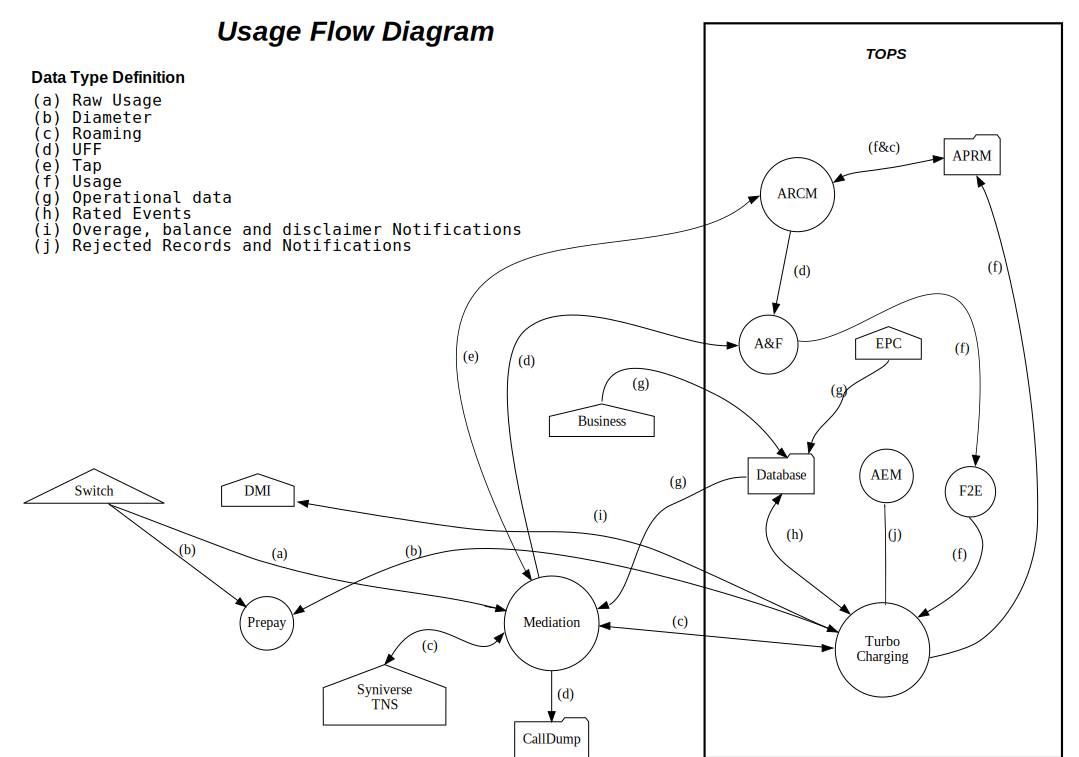
\includegraphics[width=.9\linewidth]{Pictures/uf.png}

\end{landscape} 
\newpage

\begin{landscape}  

\includegraphics[width=.9\linewidth]{Pictures/roamingPrePay.png}
\end{landscape} 
\newpage
\section{Voice Overview}
\label{sec:orgheadline12}
One major undertaking in the transition to \textbf{TOPS} is moving most of the voice mediation to the \textbf{INTEC} platform. To help facilitate this move, the current rules system \textbf{(RBMS)} was studied and documented. The following provides a brief overview of the processes used.
\subsection{Call Types}
\label{sec:orgheadline9}
\begin{enumerate}
\item \textbf{M-M} - Mobile to Mobile
\item \textbf{M-L} - Mobile to Land Line
\item \textbf{L-M} - Land Line to Mobile
\item \textbf{L-L} - Land Line to Land Line
\end{enumerate}
The call records can come in four possible states.
\begin{enumerate}
\item Mobile Terminating (Incoming)
\item Mobile Originating (Outgoing)
\item \textbf{NTI ONLY}
\begin{itemize}
\item \textbf{Both}  \newline \textbf{(NTI Mobile to Mobile)} in which for every voice event, two records are created, a \textbf{Mobile Originated} and \textbf{Mobile Terminated} record. For \textbf{APLX} this is taken care of automatically. In the case of an \textbf{NTI} switch, depending on the call scenario, it is up to the mediation platform to create one if needed.
\item \textbf{Neither} \newline (per example \textbf{L-L} )
\end{itemize}
\end{enumerate}
\includegraphics[width=11cm]{Pictures/white-charles-harvest_talk.jpg}
\newpage 
\begin{landscape}  
\subsection{Incoming - Mobile Terminated}
\label{sec:orgheadline10}
An \textbf{Incoming} call is a \emph{mobile terminated} call where one of
our customers receives a call from some caller to a \textbf{USCC}
switch.\\
\textbf{The diagram below shows the data flow for an incoming
call:} \\
\includegraphics[width=.9\linewidth]{Pictures/incoming.png}

\newpage 
\subsection{Outgoing - Mobile Originated}
\label{sec:orgheadline11}
An \textbf{outgoing} call is a \emph{mobile originating} call from a \textbf{USCC} customer in which the following can occur.\\
\textbf{The diagram below shows the data flow for an outgoing call:}
\\
\includegraphics[width=.9\linewidth]{Pictures/outgoing.png}

\end{landscape} 
\newpage

\section{Unified File Format (UFF)}
\label{sec:orgheadline18}
In \textbf{TOPs} system all \textbf{CDRs}, excluding \textbf{InCollect/OutCollect TAP or CIBER},
will be reformatted into a \emph{Unified File Format} (\textbf{UFF}). This format
is a standard \textbf{Unix/ASCII} formatted \textbf{CSV} file using '|'
\textbf{(pipe)} as the delimiter.
\subsection{UFF File Record Format}
\label{sec:orgheadline13}
\footnotesize

\begin{longtable}{c|l|l}
\hline
\textbf{Field} & \textbf{Field Name} & \textbf{Description}\\
\hline
\endfirsthead
\multicolumn{3}{l}{Continued from previous page} \\
\hline

\textbf{Field} & \textbf{Field Name} & \textbf{Description} \\

\hline
\endhead
\hline\multicolumn{3}{r}{Continued on next page} \\
\endfoot
\endlastfoot
\hline
1 & Record Type & HR - Header Record\\
 &  & DR - Data Record\\
 &  & TR - Trailer Record\\
2 & Service Type & Initial record type of Usage Record \textbf{MOT, PTX, ALU, QIS},\\
 &  & \textbf{AAA, TPC, APLX, NTI, PMG, PGW}\\
3 & Record sequence Number & A unique numeric identifier for the record.\\
4 & File Number & A unique identifier that shows the original file\\
 &  & that the record came in from. \emph{(ex. ID044803})\\
5 & Record Disposition & The disposition shows the destination of the record\\
 &  & in the Mediation process.\\
 &  & 0 = Rated\\
 &  & 1 = Dropped\\
 &  & 2 = Error\\
6 & Record Code & The Drop or Error code. The drop and error codes will be defined\\
 &  & using present day \textbf{AMDOCS} codes as a template. (presently a 3\\
 &  & digit integer but will bump to 5 for extra growth)\\
7 & Source System & Switch identifier (See Switch Name and type tab for a complete\\
 &  & listing) (Possible Voice values include:\\
 &  & madi, scha etc.) (Data values can include aaa1, vali etc.\\
8 & Start Date & Start date for this event \{YYYYMMDD\}\\
9 & Start Time & Start Time for this event \{HHMMSSss\}\\
10 & Start Time Zone & Offset in seconds from \textbf{GMT}\\
11 & Home Sid & Home Switch ID\\
12 & Serve SID & Serving Switch ID\\
13 & Originating Cell Trunk & Initial cell trunk\\
14 & Terminating Cell Trunk & Termination Cell trunk\\
15 & BSID & Broadcast Station ID\\
16 & Carrier ID & The carrier that handled the events identification symbol.\\
 &  & Mostly USCC but may contain others especially in\\
 &  & data roaming situations.\\
17 & Protocol & \textbf{EVDO, LTE, CDMA}\\
18 & Event Type & \textbf{QIS} event type used for reporting and drop logic\\
19 & Call Direction & One of two types:\\
 &  & \textbf{Mobile Originating (MO)} or \textbf{Mobile Terminating (MT)}.\\
20 & Originating MSID & 10-Digit Mobile Identification Number 16 digits for\\
 &  & possible future use/Blanks if mobile terminated\\
21 & Identity & MEID/ESN\\
22 & Originating MDN & In a Mobile Originating call It's the originating callers\\
 &  & phone number.\\
23 & Originating Address & IP or Email\\
24 & Terminating MSID & Called MSID this is on Mobile to Mobile records only.\\
25 & Terminating Number & Normalized number \emph{(example 6085551212 instead of 411}\\
26 & Dialed Digits & The untranslated dialed number \emph{(e.g. 441 instead of 555-1212)}\\
27 & Terminating Address & IP Address/Email Name Client IP for \textbf{PMG}\\
28 & Termination Code & \textbf{SMS.CALL\_TERMINATION\_CODE}\\
29 & Service Feature & MPS Service feature codes (See the list below)\\
30 & Call Forwarding Ind & If the call has been forwarded than true, false otherwise.\\
 &  & 0 = False\\
 &  & 1 = True\\
31 & Call Delivery Ind & If the call has been through call delivery than true,\\
 &  & false otherwise\\
 &  & 0 = False\\
 &  & 1 = True\\
 &  & 2 = CDLX\\
32 & Call Waiting Ind & If the call has been through call waiting than true,\\
 &  & false otherwise\\
 &  & 0 = False\\
 &  & 1 = True\\
33 & 3 way Calling Ind & If the call has been through 3 way calling, false otherwise\\
 &  & 0 = False\\
 &  & 1 = True\\
34 & Call Answered Ind & If the call has been answered than true, false otherwise.\\
 &  & 0 = False\\
 &  & 1 = True\\
35 & Ring Time & Total ring time in seconds\\
36 & Call Duration & Call duration minus ring-time in seconds.\\
 &  & Includes the duration in seconds of the data session\\
37 & Roaming Ind & Data roaming indicator 0 = False 1 = True\\
38 & Session ID & Primary Key for AAA, Transaction ID for\\
 &  & PSMS AAA.SESSION\_ID <= 64 Chars\\
 &  & PSMS.TRANS\_ID <= 50 Chars\\
 &  & QIS.EVENT\_ID <= 50 chars Used to find the charge code\\
39 & Session Type & For QIS 0 = Charge (only) For PSMS there are two possible values:\\
 &  & 0 = Charge\\
 &  & 1 = Adjustment\\
 &  & For \textbf{PTX} and \textbf{SMS} we can have the following values:\\
 &  & \textbf{SMSTXT and SMSEMIL}\\
40 & Bytes In & Total of incoming bytes associated\\
 &  & this event can also be negative.\\
 &  & Using this field and the "Bytes Out" field\\
 &  & we can derive the total bytes.\\
41 & Bytes Out & Total of outgoing bytes associated with this event contains\\
 &  & a signed byte (+-) Using this field and the "Bytes In" field\\
 &  & we can derive the total bytes.\\
42 & Application ID & QIS = Part ID AAA = AppID PSMS = Short Code\\
43 & Application Type & QIS = (Download or Subscription) PSMS = (One-Off or Subscription)\\
44 & Application Name & \\
45 & Purchase Category Code & Used by PSMS\\
46 & Application Description & Will be used for both QIS and PSMS for QIS it will come from the\\
 &  & AE field directly on the record for PSMS it will be a\\
 &  & combination of the <short code> <description> <content provider>\\
 &  & if it is a "Subscription", "Subscription -" is displayed.\\
 &  & If it is a one-off, it is not\\
 &  & presented in the invoice line item.\\
47 & Content Amount & Combines Pre-rated usage amount for QIS and PSMS\\
48 & Orig\_trans\_ID & Orig Trans ID PSMS.TRANS\_ID\\
49 & Network Flag & Used by QIS to calculate the charge code.\\
 &  & 0 = not a 1 = is a network application..\\
 &  & Default is 0\\
50 & Femto-cell-ringtime & Will not be needed until after \textbf{TOPS} implementation\\
51 & Femto-cell-ringpluse & Will not be needed until after \textbf{TOPS} implementation\\
52 & LTE Handoff & This maybe needed after the move to LTE,\\
 &  & so is just used as a placeholder\\
53 & Market/Sub-market & The Market and Sub-market for a customer this can also be blank.\\
 &  & This field is populated by using a MSID against the MIN\_LR\\
54 & Originating IMSI & The IMSI assigned to the SIM card originating a LTE or eHRPD\\
 &  & data session. This can be a routing parameter\\
 &  & for LTE or eHRPD traffic.\\
55 & Adjustment Reason Code & The Adjustment Reason Code for a PSMS adjustment\\
56 & External Reference ID & The External Reference ID for a PSMS record\\
57 & Partner ID & The Partner ID for PSMS record\\
58 & Campaign ID & The Campaign ID for a PSMS record\\
59 & Initiator Type & The Initiator Type for PSMS record\\
60 & Initiator ID & The Initiator ID for PSMS record\\
\hline
\end{longtable}
\normalsize
\subsection{Header}
\label{sec:orgheadline14}
\footnotesize

\begin{longtable}{c|l|l|l}
\hline
\textbf{Field} & \textbf{Field Name} & \textbf{Description} & \textbf{Data Type}\\
\hline
\endfirsthead
\multicolumn{4}{l}{Continued from previous page} \\
\hline

\textbf{Field} & \textbf{Field Name} & \textbf{Description} & \textbf{Data Type} \\

\hline
\endhead
\hline\multicolumn{4}{r}{Continued on next page} \\
\endfoot
\endlastfoot
\hline
1 & Record Type & The record type for Header is HR & 4 character alpha-numeric\\
 &  &  & \\
2 & File Number & file Identifier A unique identifier & alpha-numeric <= 24 chars and\\
 &  & that shows the original file that & have the pattern IDxxxxxxx..\\
 &  & the record name in from. (ex. ID044803) & Where xxxx is a number that's\\
 &  &  & no greater then 16 char\\
 &  &  & \\
3 & Source System & Switch identifier (See Switch Name & alpha-numeric <= 16 characters\\
 &  & and type tab for a complete listing) & \\
 &  & (Possible Voice values include: madi, & \\
 &  & scha etc.) (Data values can include & \\
 &  & aaa1, vali etc. & \\
 &  &  & \\
4 & Start Date & Start date of file creation \{YYYYMMDD\} & Event Date YYYYMMDD\\
 &  &  & 1900 <= YYYY <=9999\\
 &  &  & 01 <= MM <= 12\\
 &  &  & 01 <= DD <= 31\\
 &  &  & \\
5 & Start Time & Start Time for file creation \{HHMMSSss\} & Switch Time HHMMSSss\\
 &  &  & 00 <= HH <= 23\\
 &  &  & 00 <= MM <= 59\\
 &  &  & 00 <= SS <= 59\\
 &  &  & 00 <= ss <= 59\\
\hline
\end{longtable}
\normalsize
\newpage
\subsection{Trailer}
\label{sec:orgheadline15}
\footnotesize

\begin{longtable}{c|l|l|l}
\hline
\textbf{Field} & \textbf{Field Name} & \textbf{Description} & \textbf{Data Type}\\
\hline
\endfirsthead
\multicolumn{4}{l}{Continued from previous page} \\
\hline

\textbf{Field} & \textbf{Field Name} & \textbf{Description} & \textbf{Data Type} \\

\hline
\endhead
\hline\multicolumn{4}{r}{Continued on next page} \\
\endfoot
\endlastfoot
\hline
1 & Record Type & The record type for Trailer is TR & 4 character alpha-numeric\\
 &  &  & \\
2 & File Number & File Identifier A unique identifier & alpha-numeric <= 24 chars and have the\\
 &  & that shows the original file that & pattern IDxxxxxxx.. Where xxxx is\\
 &  & the record came in from. (ex. ID044803) & a number that's no greater then 16 char\\
 &  &  & \\
3 & Source System & Switch identifier (See Switch Name & alpha-numeric <= 16 chars\\
 &  & and type tab for a complete listing) & \\
 &  & (Data values can include aaa1, vali etc. & \\
 &  &  & \\
4 & End Date & End date of file creation \{YYYYMMDD\} & Event Date YYYYMMDD\\
 &  &  & 1900 <= YYYY <=9999\\
 &  &  & 01 <= MM <= 12\\
 &  &  & 01 <= DD <= 31\\
 &  &  & \\
5 & End Time & End Time of file creation \{HHMMSSss\} & Switch Time HHMMSSss\\
 &  &  & 00 <= HH <= 23\\
 &  &  & 00 <= MM <= 59\\
 &  &  & 00 <= SS <= 59\\
 &  &  & 00 <= ss <= 59\\
 &  &  & \\
6 & Total Records & Total number of records in this file & numeric <= 100000000\\
 &  &  & (Including Header and trailers)\\
\hline
\end{longtable}
\normalsize
\subsection{Service Feature Codes}
\label{sec:orgheadline16}
Description of the service feature codes found in field 29 of the \textbf{UFF}
\footnotesize
\begin{longtable}{l|l}
\hline
\textbf{Description} & \textbf{Code}\\
\hline
\endfirsthead
\multicolumn{2}{l}{Continued from previous page} \\
\hline

\textbf{Description} & \textbf{Code} \\

\hline
\endhead
\hline\multicolumn{2}{r}{Continued on next page} \\
\endfoot
\endlastfoot
\hline
(NTI Only) - Automatic Roaming & ARM\\
Call Delivery Interconnect & CDLX\\
Call Forward Immediate & CFW\\
Call Forward Busy & CFB\\
Call Forward No Answer Transfer & CFWTRN\\
(NTI Only) - Calls to/from hotline & HT\\
(NTI Only) -Inter system hand-off & ISH\\
Operator assisted call & OPA\\
(NTI Only) - Vertical feature flag & VFF\\
Voice-mail delivery & VMD\\
Voice-mail retrieval & VMR\\
Caller ID Restriction (ID block) & CIR\\
\hline
\end{longtable}
\normalsize
\subsection{\href{docs/Drop\%20Reason\%20Codes.pdf}{Drop Reason Codes}}
\label{sec:orgheadline17}
There many many reasons why a record can be dropped and are to numerous to list. The complete list can forwarded upon request.

\newpage
\section{CIBER File Format}
\label{sec:orgheadline27}
Incollect and Outcollect \textbf{CDMA} files are come in the \textbf{CIBER} File format which is a fixed length record format described below.
\subsection{Ciber Record Types}
\label{sec:orgheadline24}
The \textbf{Ciber} standard defines the following record Types:
\begin{itemize}
\item \textbf{01} Header
\item \textbf{22} Voice (main Record type)
\item \textbf{32} Data
\item \textbf{52} One time charge
\item \textbf{98} Trailer
\end{itemize}

\subsubsection{CIBER 01 Record}
\label{sec:orgheadline19}
\footnotesize

\begin{longtable}{l|l|l}
\hline
\textbf{Field} & \textbf{Position} & \textbf{Description}\\
\hline
\endfirsthead
\multicolumn{3}{l}{Continued from previous page} \\
\hline

\textbf{Field} & \textbf{Position} & \textbf{Description} \\

\hline
\endhead
\hline\multicolumn{3}{r}{Continued on next page} \\
\endfoot
\endlastfoot
\hline
Record Type & 1-2 & \\
Batch Creation Date & 3-8 & \\
Batch Sequence Number & 9-11 & \\
Sending Carrier SID/BID & 12-16 & \\
Receiving Carrier SID/BID & 17-21 & \\
CIBER Record Release Number & 22-23 & \\
Original/Return Indicator & 24-24 & \\
Currency Type & 25-26 & \\
Settlement Period & 27-32 & \\
Clearinghouse ID & 33-33 & \\
CIBER Batch Reject Reason Code & 34-35 & \\
Batch Contents & 36-36 & \\
Local Carrier Reserved & 37-56 & \\
System Reserved Filler & 57-200 & \\
\hline
\end{longtable}

\normalsize
\newpage 
\subsubsection{CIBER 22 Record}
\label{sec:orgheadline20}
Voice roaming record.
\footnotesize

\begin{longtable}{l|l|l}
\hline
\textbf{FIELD NAME} & \textbf{POSITION} & \textbf{Description}\\
\hline
\endfirsthead
\multicolumn{3}{l}{Continued from previous page} \\
\hline

\textbf{FIELD NAME} & \textbf{POSITION} & \textbf{Description} \\

\hline
\endhead
\hline\multicolumn{3}{r}{Continued on next page} \\
\endfoot
\endlastfoot
\hline
Record Type & 1-2 & \\
Return Code & 3-3 & \\
CIBER Record Return Reason Code & 4-5 & \\
Invalid Field Identifier & 6-8 & \\
Home Carrier SID/BID & 9-13 & \\
MSID Indicator & 14-14 & \\
\textbf{MSID} & 15-29 & \\
MSISDN/MDN Length & 30-31 & \\
\textbf{MSISDN/MDN} & 32-46 & \\
\textbf{ESN/UIMID/IMEI/MEID Indicator} & 47-47 & 0 = NA\\
 &  & 1 = ESN\\
 &  & 2 = IMEI\\
 &  & 3 = MEID\\
 &  & 4 = pESN\\
\textbf{ESN/UIMID/IMEI/MEID} & 48-66 & \\
\textbf{Serving Carrier SID/BID} & 67-71 & \\
\textbf{Total Charges and Taxes} & 72-81 & \\
System Reserved Filler & 82-82 & \\
\textbf{Total State/Province Taxes} & 83-92 & \\
System Reserved Filler & 93-93 & \\
\textbf{Total Local/Other Taxes} & 94-103 & \\
System Reserved Filler & 104-104 & \\
\textbf{Call Date} & 105-110 & \\
\textbf{Call Direction} & 111-111 & \\
Call Completion Indicator & 112-112 & \\
Call Termination Indicator & 113-113 & \\
Caller ID Length & 114-115 & \\
Caller ID & 116-130 & \\
Called Number Length & 131-132 & \\
\textbf{Called Number Digits} & 133-147 & \\
Location Routing Number Length Indicator & 148-149 & \\
Location Routing Number & 150-164 & \\
TLDN Length & 165-166 & \\
TLDN & 167-181 & \\
Currency Type & 182-183 & \\
System Reserved Filler & 184-185 & \\
Original Batch Sequence Number & 186-188 & \\
Initial Cell Site & 189-199 & \\
Time Zone Indicator & 200-201 & \\
Daylight Savings Indicator & 202-202 & \\
Message Accounting Digits & 203-212 & \\
Air Connect Time & 213-218 & \\
Air Chargeable Time & 219-224 & \\
Air Elapsed Time & 225-230 & \\
Air Rate Period & 231-232 & \\
Air Multi-Rate Period & 233-233 & \\
\textbf{Air Charge} & 234-243 & \\
System Reserved Filler & 244-244 & \\
Other Charge No. 1 Indicator & 245-246 & \\
\textbf{Other Charge No. 1} & 247-256 & \\
System Reserved Filler & 257-257 & \\
System Reserved Filler & 258-270 & \\
Printed Call & 271-285 & \\
Fraud Indicator & 286-287 & \\
Fraud Sub-Indicator & 288-288 & \\
\textbf{Special Features Used} & 289-293 & \\
\textbf{Called Place} & 294-303 & \\
\textbf{Called State/Province} & 304-305 & \\
\textbf{Called Country} & 306-308 & \\
\textbf{Serving Place} & 309-318 & \\
\textbf{Serving State/Province} & 319-320 & \\
\textbf{Serving Country} & 321-323 & \\
Toll Connect Time & 324-329 & \\
Toll Chargeable Time & 330-335 & \\
Toll Elapsed Time & 336-341 & \\
Toll Tariff Descriptor & 342-343 & \\
Toll Rate Period & 344-345 & \\
Toll Multi-Rate Period & 346-346 & \\
Toll Rate Class & 347-347 & \\
Toll Rating Point Length Indicator & 348-349 & \\
Toll Rating Point & 350-359 & \\
\textbf{Toll Charge} & 360-369 & \\
System Reserved Filler & 370-370 & \\
\textbf{Toll State/Province Taxes} & 371-380 & \\
System Reserved Filler & 381-381 & \\
\textbf{Toll Local Taxes} & 382-391 & \\
System Reserved Filler & 392-392 & \\
Toll Network Carrier ID & 393-397 & \\
Local Carrier Reserved & 398-472 & \\
System Reserved Filler & 473-547 & \\
\hline
\end{longtable}
\normalsize
\subsubsection{CIBER 32 Record}
\label{sec:orgheadline21}
Data roaming record.
\footnotesize

\begin{longtable}{l|l|l}
\hline
\textbf{Field} & \textbf{Position} & \textbf{Description}\\
\hline
\endfirsthead
\multicolumn{3}{l}{Continued from previous page} \\
\hline

\textbf{Field} & \textbf{Position} & \textbf{Description} \\

\hline
\endhead
\hline\multicolumn{3}{r}{Continued on next page} \\
\endfoot
\endlastfoot
\hline
Record Type & 1-2 & \\
Return Code & 3-3 & \\
CIBER Record Return Reason Code & 4-5 & \\
Invalid Field Identifier & 6-8 & \\
Home Carrier SID/BID & 9-13 & \\
MSID Indicator & 14-14 & \\
MSID & 15-29 & \\
MSISDN/MDN Length & 30-31 & \\
MSISDN/MDN & 32-46 & \\
ESN/UIMID/IMEI/MEID Indicator & 47-47 & \\
ESN/UIMID/IMEI/MEID & 48-66 & \\
Serving Carrier SID/BID & 67-71 & \\
Total Charges and Taxes & 72-81 & \\
System Reserved Filler & 82-82 & \\
Total State/Province Taxes & 83-92 & \\
System Reserved Filler & 93-93 & \\
Total Local Taxes & 94-103 & \\
System Reserved Filler & 104-104 & \\
Call Date & 105-110 & \\
Call Direction & 111-111 & \\
Call Completion Indicator & 112-112 & \\
Call Termination Indicator & 113-113 & \\
Caller ID Length & 114-115 & \\
Caller ID & 116-130 & \\
Called Number Length & 131-132 & \\
Called Number Digits & 133-147 & \\
Location Routing Number Length Indicator & 148-149 & \\
Location Routing Number & 150-164 & \\
TLDN Length & 165-166 & \\
TLDN & 167-181 & \\
Currency Type & 182-183 & \\
System Reserved Filler & 184-185 & \\
Original Batch Sequence Number & 186-188 & \\
Initial Cell Site & 189-199 & \\
Time Zone Indicator & 200-201 & \\
Daylight Savings Indicator & 202-202 & \\
Message Accounting Digits & 203-212 & \\
Charge No. 1 Indicator & 213-214 & \\
Charge No. 1 Connect Time & 215-220 & \\
Charge No. 1 Chargeable Time & 221-226 & \\
Charge No. 1 Elapsed Time & 227-232 & \\
Charge No. 1 Rate Period & 233-234 & \\
Charge No. 1 Multi-Rate Period & 235-235 & \\
Charge No. 1 Tax/Surcharge Indicator & 236-236 & \\
Charge No. 1 & 237-246 & \\
System Reserved Filler & 247-247 & \\
Charge No. 2 Indicator & 248-249 & \\
Charge No. 2 Connect Time & 250-255 & \\
Charge No. 2 Chargeable Time & 256-261 & \\
Charge No. 2 Elapsed TIme & 262-267 & \\
Charge No. 2 Rate Period & 268-269 & \\
Charge No. 2 Multi-Rate Period & 270-270 & \\
Charge No. 2 Tax/Surcharge Indicator & 271-271 & \\
Charge No. 2 & 272-281 & \\
System Reserved Filler & 282-282 & \\
Charge No. 3 Indicator & 283-284 & \\
Charge No. 3 Connect Time & 285-290 & \\
Charge No. 3 Chargeable Time & 291-296 & \\
Charge No. 3 Elapsed Time & 297-302 & \\
Charge No. 3 Rate Period & 303-304 & \\
Charge No. 3 Multi-Rate Period & 305-305 & \\
Charge No. 3 Tax/Surcharge Indicator & 306-306 & \\
Charge No. 3 & 307-316 & \\
System Reserved Filler & 317-317 & \\
Charge No. 4 Indicator & 318-319 & \\
Charge No. 4 Connect Time & 320-325 & \\
Charge No. 4 Chargeable Time & 326-331 & \\
Charge No. 4 Elapsed Time & 332-337 & \\
Charge No. 4 Rate Period & 338-339 & \\
Charge No. 4 Multi-Rate Period & 340-340 & \\
Charge No. 4 Tax/Surcharge Indicator & 341-341 & \\
Charge No. 4 & 342-351 & \\
System Reserved Filler & 352-352 & \\
Blank Fill Serving Place & 353-362 & \\
Serving State/Province & 363-364 & \\
Serving Country & 365-367 & \\
Special Features Used & 368-372 & \\
Other Charge No. 1 Indicator & 373-374 & \\
Other Charge No. 1 & 375-384 & \\
System Reserved Filler & 385-385 & \\
System Reserved Filler & 386-398 & \\
Printed Call & 399-413 & \\
Fraud Indicator & 414-415 & \\
Fraud Sub-Indicator & 416-416 & \\
Features Used After Handoff Indicator & 417-417 & \\
Local Carrier Reserved & 418-492 & \\
System Reserved Filler & 493-567 & \\
\hline
\end{longtable}
\normalsize

\subsubsection{CIBER 52 Record}
\label{sec:orgheadline22}
\footnotesize

\begin{longtable}{l|l|l}
\hline
\textbf{FIELD} & \textbf{POSITION} & \textbf{Description}\\
\hline
\endfirsthead
\multicolumn{3}{l}{Continued from previous page} \\
\hline

\textbf{FIELD} & \textbf{POSITION} & \textbf{Description} \\

\hline
\endhead
\hline\multicolumn{3}{r}{Continued on next page} \\
\endfoot
\endlastfoot
\hline
Return Code & 3-3 & \\
CIBER Record Return Reason Code & 4-5 & \\
Invalid Field Identifier & 6-8 & \\
Home Carrier SID/BID & 9-13 & \\
MSID Indicator & 14-14 & \\
\textbf{MSID} & 15-29 & \\
MSISDN/MDN Length & 30-31 & \\
MSISDN/MDN & 32-46 & \\
ESN/UIMID/IMEI/MEID Indicator & 47-47 & \\
ESN/UIMID/IMEI/MEID & 48-66 & \\
Serving Carrier SID/BID & 67-71 & \\
\textbf{Total Charges and Taxes} & 72-81 & \\
System Reserved Filler & 82-82 & \\
\textbf{Total State/Province Taxes} & 83-92 & \\
System Reserved Filler & 93-93 & \\
\textbf{Total Local Taxes} & 94-103 & \\
System Reserved Filler & 104-104 & \\
\textbf{OCC Charge/Start Date} & 105-110 & \\
Connect Time & 111-116 & \\
OCC End Date & 117-122 & \\
OCC Interval Indicator & 124-133 & \\
\textbf{OCC Charge} & 134-134 & \\
System Reserved Filler & 135-159 & \\
OCC Description Currency Type & 160-161 & \\
System Reserved Filler & 123-123 & \\
Original Batch Sequence Number & 164-166 & \\
Initial Cell Site & 167-177 & \\
Time Zone Indicator & 178-179 & \\
Daylight Savings Indicator & 180-180 & \\
Message Accounting Digits & 181-190 & \\
Record Use Indicator & 191-191 & \\
Serving Place & 192-201 & \\
Serving State/Province & 202-203 & \\
Serving Country & 204-206 & \\
Other Charge No. 1 Indicator & 207-208 & \\
Other Charge No. 1 & 209-218 & \\
System Reserved Filler & 219-219 & \\
System Reserved Filler & 220-232 & \\
Fraud Indicator & 233-234 & \\
Fraud Sub-Indicator & 235-235 & \\
Record Create Date & 236-241 & \\
System Reserved Filler & 220-232 & \\
Fraud Indicator & 233-234 & \\
Fraud Sub-Indicator & 235-235 & \\
Record Create Date & 236-241 & \\
\hline
\end{longtable}
\normalsize
\newpage
\subsubsection{CIBER 98 Record}
\label{sec:orgheadline23}
\footnotesize

\begin{longtable}{l|l|l}
\hline
\textbf{FIELD} & \textbf{POSITION} & \textbf{Description}\\
\hline
\endfirsthead
\multicolumn{3}{l}{Continued from previous page} \\
\hline

\textbf{FIELD} & \textbf{POSITION} & \textbf{Description} \\

\hline
\endhead
\hline\multicolumn{3}{r}{Continued on next page} \\
\endfoot
\endlastfoot
\hline
Record Type & 1-2 & \\
Batch Creation Date & 3-8 & \\
Batch Sequence Number & 9-11 & \\
Sending Carrier SID/BID & 12-16 & \\
Receiving Carrier SID/BID & 17-21 & \\
\textbf{Total Number Records in Batch} & 22-25 & \\
\textbf{Batch Total Charges \& Taxes} & 26-37 & \\
Settlement Period & 38-43 & \\
Clearinghouse ID & 44-44 & \\
System Reserved Filler & 45-49 & \\
Original Total Number of Records & 50-53 & \\
\textbf{Original Total Charges \& Taxes} & 54-65 & \\
System Reserved Filler & 66-73 & \\
Currency Type & 74-75 & \\
Local Carrier Reserved & 76-95 & \\
System Reserved Filler & 96-200 & \\
\hline
\end{longtable}
\normalsize
\subsection{MF1\_CIBER\_BATCH\_SEQ}
\label{sec:orgheadline25}
The table used to keep the CIBER Outcollect sequences in sync
with Syniverse. Every once a while we need to update it to keep
in sync.

\href{file:///home/dbalchen/workspace/Outcollects/updateSeq.pl}{Sequence Creation Job}

\footnotesize
\begin{longtable}{l|l|l}
\hline
\textbf{Column Name} & \textbf{Data Type} & \textbf{Description}\\
\hline
\endfirsthead
\multicolumn{3}{l}{Continued from previous page} \\
\hline

\textbf{Column Name} & \textbf{Data Type} & \textbf{Description} \\

\hline
\endhead
\hline\multicolumn{3}{r}{Continued on next page} \\
\endfoot
\endlastfoot
\hline
Application\_Id & Char (6 Byte) & \\
Dl\_Service\_Code & Char (5 Byte) & \\
Dl\_Update\_Stamp & Number (4) & \\
\textbf{Home\_Sid} & Char (5 Byte) & \\
Locked\_Sid & Number (10) & \\
Operator\_Id & Number (9) & \\
Seq\_No & Number (3) & \\
\textbf{Serve\_Sid} & Char (5 Byte) & \\
Status\_Ind & Char (2 Byte) & \\
Sys\_Creation\_Date & Date & \\
Sys\_Update\_Date & Date & \\
\hline
\end{longtable}
\normalsize
\subsection{CIBERNET - Specification/Reference}
\label{sec:orgheadline26}
\url{https://www.one1clear.net/mxp/Login.asp} 

\newpage 

\section{Acquisition and Formating (A\&F)}
\label{sec:orgheadline31}
\textbf{A\&F} is the first stage of the \textbf{TOPS} mediation process where the \textbf{UFF} or \textbf{CIBER} record is examined, enriched 
and transfered to an intermediary \emph{usage} format. For \textbf{CIBER} records an extra rules step is 
added to further mediate the records.
\subsection{AC\_PHYSICAL\_FILES}
\label{sec:orgheadline28}
Provides information for the physical files that were processed.
\footnotesize

\begin{longtable}{l|l|l}
\hline
\textbf{Column Name} & \textbf{Data Type} & \textbf{Description}\\
\hline
\endfirsthead
\multicolumn{3}{l}{Continued from previous page} \\
\hline

\textbf{Column Name} & \textbf{Data Type} & \textbf{Description} \\

\hline
\endhead
\hline\multicolumn{3}{r}{Continued on next page} \\
\endfoot
\endlastfoot
\hline
\textbf{Identifier} & Number(15,0) & file Identifier\\
\textbf{Sys\_Creation\_Date} & Date & \\
Sys\_Update\_Date & Date & \\
Operator\_Id & Number(9,0) & \\
Application\_Id & Char(6 Byte) & \\
Dl\_Service\_Code & Char(5 Byte) & \\
Dl\_Update\_Stamp & Number(4,0) & \\
\textbf{File\_Name} & Varchar2(200 Byte) & \\
Host\_Name & Varchar2(50 Byte) & \\
\textbf{File\_Path} & Varchar2(512 Byte) & \\
Serial\_Number & Varchar2(8 Byte) & \\
System\_Rcv\_Date & Date & \\
Fsrc\_Src\_Type & Char(10 Byte) & \\
Fsrc\_Type\_Id & Char(10 Byte) & \\
Rcrdng\_Start\_Date & Date & \\
Rcrdng\_End\_Date & Date & \\
\textbf{Trlr\_Record\_Count} & Number(9,0) & \\
Trlr\_Block\_Count & Number(9,0) & \\
Trlr\_L\_File\_Count & Number(9,0) & \\
Pgm\_L\_File\_Count & Number(9,0) & \\
Pgm\_Tracer\_Ind & Char(1 Byte) & \\
Dupl\_Entry\_Ind & Char(1 Byte) & \\
Entry\_Status & Char(2 Byte) & \\
Old\_Age\_Ind & Char(1 Byte) & \\
End\_Of\_Tree\_Seq & Number(9,0) & \\
\textbf{Balance\_Date} & Date & \\
\hline
\end{longtable}
\normalsize
\subsection{AC\_SOURCE}
\label{sec:orgheadline29}
This table lists the \textbf{network elements} and the file type processed. When a new network element is created, an entry describing it must be created.
\footnotesize

\begin{longtable}{l|l|l}
\hline
\textbf{Column Name} & \textbf{Data Type} & \textbf{Description}\\
\hline
\endfirsthead
\multicolumn{3}{l}{Continued from previous page} \\
\hline

\textbf{Column Name} & \textbf{Data Type} & \textbf{Description} \\

\hline
\endhead
\hline\multicolumn{3}{r}{Continued on next page} \\
\endfoot
\endlastfoot
\hline
Source\_Type & Char(10 Byte) & \\
\textbf{File\_Type} & Char(10 Byte) & UFF/CIBER etc.\\
\textbf{Switch\_Id} & Varchar2(32 Byte) & Network Element\\
Sys\_Creation\_Date & Date & \\
Sys\_Update\_Date & Date & \\
Operator\_Id & Number(9,0) & \\
Application\_Id & Char(6 Byte) & \\
Dl\_Service\_Code & Char(5 Byte) & \\
Dl\_Update\_Stamp & Number(4,0) & \\
File\_Seq\_No & Number(6,0) & \\
Max\_File\_Seq\_No & Number(6,0) & \\
Max\_Time & Number(10,0) & \\
Min\_Time & Number(10,0) & \\
Last\_Cycle\_Procd & Date & \\
Next\_Cycle\_Expect & Date & \\
Status\_Ind & Char(2 Byte) & \\
Dupl\_Entry\_Ind & Char(1 Byte) & \\
Ho\_From\_Time & Date & \\
Ho\_From\_Seq & Number(6,0) & \\
Days\_Bfr\_Phy\_Cln & Number(4,0) & \\
Gap\_Permitted & Number(6,0) & \\
\hline
\end{longtable}

\subsection{AC1\_CONTROL (-HIST)}
\label{sec:orgheadline30}
When it comes to investigating usage issues \textbf{AC1\_CONTROL\_HIST} in both \textbf{PRDAF} (Usage) \textbf{PRDCUST} (AR) is usually the first stop for any file issues.


\footnotesize

\begin{longtable}{l|l|l}
\hline
\textbf{Column Name} & \textbf{Data Type} & Description\\
\hline
\endfirsthead
\multicolumn{3}{l}{Continued from previous page} \\
\hline

\textbf{Column Name} & \textbf{Data Type} & Description \\

\hline
\endhead
\hline\multicolumn{3}{r}{Continued on next page} \\
\endfoot
\endlastfoot
\hline
\textbf{Identifier} & Number(15,0) & \\
Sys\_Creation\_Date & Date & \\
Sys\_Update\_Date & Date & \\
Operator\_Id & Number(9,0) & \\
Application\_Id & Char(6 Byte) & \\
Dl\_Service\_Code & Char(5 Byte) & \\
Dl\_Update\_Stamp & Number(4,0) & \\
\textbf{File\_Name} & Varchar2(200 Byte) & \\
\textbf{File\_Path} & Varchar2(512 Byte) & \\
File\_Seq\_No & Number(6,0) & \\
Host\_Name & Varchar2(50 Byte) & \\
Data\_Group & Varchar2(64 Byte) & \\
File\_Create\_Date & Date & \\
\textbf{File\_Status} & Varchar2(2 Byte) & \\
\textbf{Origin\_File\_Ident} & Number(15,0) & The Identifier of\\
 &  & the original file.\\
\textbf{Phy\_File\_Ident} & Number(15,0) & \\
Cur\_Pgm\_Name & Varchar2(32 Byte) & \\
Cur\_File\_Alias & Varchar2(10 Byte) & \\
Nxt\_Pgm\_Name & Varchar2(32 Byte) & \\
Nxt\_File\_Alias & Varchar2(10 Byte) & \\
File\_Format & Varchar2(10 Byte) & \\
File\_Group & Char(1 Byte) & \\
File\_Type & Char(2 Byte) & \\
Repro\_Ind & Char(1 Byte) & \\
Source\_Type & Char(10 Byte) & \\
Source\_File\_Type & Char(10 Byte) & \\
File\_Deleted\_Ind & Char(1 Byte) & \\
System\_Id & Char(5 Byte) & \\
Abp\_Var & Varchar2(512 Byte) & \\
Priority & Char(1 Byte) & \\
Wr\_Rec\_Quantity & Number(9,0) & \\
Wr\_Time\_Quantity & Number(13,2) & \\
Wr\_Money\_Quantity & Number(13,2) & \\
Wr\_Euro\_Quantity & Number(13,2) & \\
In\_Rec\_Quantity & Number(9,0) & \\
In\_Time\_Quantity & Number(13,2) & \\
In\_Money\_Quantity & Number(13,2) & \\
In\_Euro\_Quantity & Number(13,2) & \\
Gn\_Rec\_Quantity & Number(9,0) & \\
Gn\_Time\_Quantity & Number(13,2) & \\
Gn\_Money\_Quantity & Number(13,2) & \\
Gn\_Euro\_Quantity & Number(13,2) & \\
Dr\_Rec\_Quantity & Number(9,0) & \\
Dr\_Time\_Quantity & Number(13,2) & \\
Dr\_Money\_Quantity & Number(13,2) & \\
Dr\_Euro\_Quantity & Number(13,2) & \\
Processed\_Rec\_No & Number(9,0) & \\
Rejected\_Reason\_Cd & Char(3 Byte) & \\
Owner\_Name & Varchar2(50 Byte) & \\
Table\_Alias & Number(5,0) & \\
Nxt\_Process\_Id & Number(9,0) & \\
Nxt\_Process\_Start\_Time & Date & \\
Cur\_Process\_Id & Number(9,0) & \\
Max\_Event\_Time & Date & \\
Logical\_File\_Ident & Number(15,0) & \\
Table\_Issue\_Code & Number(9,0) & \\
External\_Id & Varchar2(32 Byte) & \\
Dest\_Rout\_Crtria & Varchar2(24 Byte) & \\
Status\_Category & Varchar2(20 Byte) & \\
Status\_Code & Varchar2(200 Byte) & \\
Application\_Code & Varchar2(50 Byte) & \\
File\_Size & Number(15,0) & \\
Recycle\_Counter & Number(15,0) & \\
Group\_Sequence & Number(15,0) & \\
Out\_Req\_Quantity & Number(9,0) & \\
Bulk\_Id & Number(9,0) & \\
Store\_Mode & Char(2 Byte) & \\
Session\_Id & Number(15,0) & \\
Target\_File\_Path & Varchar2(512 Byte) & \\
Target\_Host & Varchar2(50 Byte) & \\
Ext\_Identifier & Number(9,0) & \\
Ext\_Orig\_Ident & Number(9,0) & \\
Additional\_Attr & Varchar2(300 Byte) & \\
Group\_Size & Number(4,0) & \\
Monitor\_Data & Varchar2(50 Byte) & \\
Wr\_Volume\_Quantity & Number(15,2) & \\
In\_Volume\_Quantity & Number(15,2) & \\
Gn\_Volume\_Quantity & Number(15,2) & \\
Dr\_Volume\_Quantity & Number(15,2) & \\
End\_Process\_Time & Date & \\
Fr\_Time & Date & \\
Eng\_Priority & Number(1,0) & \\
\hline
\end{longtable}
\newpage 
\section{TurboCharging}
\label{sec:orgheadline67}
   The most important \emph{sub-system} in \textbf{TOPS}. It is here that all usage is guided and rated.
\\
\\
\includegraphics[width=16cm]{Pictures/TC.png}
\begin{itemize}
\item \textbf{Event flow:}
\begin{enumerate}
\item An event comes in to via a network element
\item Transforms data into a conical form which also includes the
network element.
\item Gets Rated
\begin{itemize}
\item For \textbf{Pre-Pay} the \textbf{HLR\footnote{Home Location Resource}}. is handled by the \textbf{SCP\footnote{Service Control Protocol}}
\item We convert everything to the customers \textbf{Home SID timezone} for bill
presentment.
\item Limiting or "\emph{choking}" usage can be handled by \textbf{Diameter\footnote{Application which implements the \textbf{SCP} Protocol}} for
\textbf{Pre-Pay} and \textbf{Turbo-Charging} for \textbf{Post-Pay}
\end{itemize}
\end{enumerate}
\end{itemize}
\subsection{Guide By Criteria}
\label{sec:orgheadline32}
The value used for each usage type to find the customer information. 
\begin{center}
\begin{tabular}{ll}
\hline
\textbf{Data Types} & \textbf{Guide By}\\
\hline
voice & MSID\\
GSM & \textbf{IMSI}\\
SMS & MDN\\
VOLTE/TAS & IMSI\\
PMG/PTX & MSID\\
AAA & MSID\\
\textbf{PGW/LTE} & \textbf{MDN/IMSI}\\
Vali & MDN\\
\hline
\end{tabular}
\end{center}
\subsection{Event Servers}
\label{sec:orgheadline33}
\textbf{Turbo-Charging} is not one application but multiple instances of \textbf{Event Servers}. Each event server corresponds to a bill cycle. Their status can be viewed using
     the following query on the \textbf{PRDAF} database.
\begin{verbatim}
 SELECT DISTINCT
         A.PROCESS_GROUP_ID,
         PROCESS_CODE,
         DECODE (HOST_ID,
                 2001, 'EVESRV1',
                 2022, 'EVESRV2',
                 2023, 'EVESRV3',
                 2024, 'EVESRV4',
                 2025, 'EVESRV5',
                 2026, 'EVESRV6')
             AS "MACHINE",
         DESCRIPTION,
         DECODE (PROCESS_GROUP_ROLE,  0, 'ACTIVE',  1, 'STANDBY') ES_STATUS
    FROM AVM1_SEGMENT_TOPOLOGY A, GN1_SYS_PROC_INSTANCE_CFG B
   WHERE     A.PROCESS_GROUP_ID = B.PROCESS_GROUP_ID
         AND A.ACTIVE_PROCESS_ID = B.PROCESS_INSTANCE_ID
         AND PROCESS_CODE LIKE '%ES1%'
ORDER BY MACHINE ASC
\end{verbatim}
\subsection{Rerate Servers}
\label{sec:orgheadline34}
In addition we have five \textbf{Rerate Servers} they are:
\begin{center}
\begin{tabular}{ll}
1. \textbf{RRP\_EOC1056} & 4. \textbf{RRP\_EOC1257}\\
2. \textbf{RRP\_EOC1068} & 5. \textbf{RRP\_EOC1259}\\
3. \textbf{RRP\_EOC1192} & \\
\end{tabular}
\end{center}


\normalsize
\newpage 
\subsection{AGD1\_RESOURCES}
\label{sec:orgheadline35}
Given a customer attribute, use this table to find the rest of the customer information.
\footnotesize

\begin{longtable}{l|l|l}
\hline
\textbf{Column Name} & \textbf{Data Type} & \textbf{Description}\\
\hline
\endfirsthead
\multicolumn{3}{l}{Continued from previous page} \\
\hline

\textbf{Column Name} & \textbf{Data Type} & \textbf{Description} \\

\hline
\endhead
\hline\multicolumn{3}{r}{Continued on next page} \\
\endfoot
\endlastfoot
\hline
Resource\_Segment & Number(4,0) & \\
Resource\_Value & Varchar2(63 Byte) & Contains\\
\textbf{Resource\_Type} & Number(4,0) & 0 - Mdn\\
 &  & 19 - Min\\
 &  & 21 - Outcollects\\
 &  & 23 - Timsi\\
\textbf{Effective\_Date} & Date & \\
Sys\_Creation\_Date & Date & \\
Sys\_Update\_Date & Date & \\
Operator\_Id & Number(9,0) & \\
Application\_Id & Char(6 Byte) & \\
Dl\_Service\_Code & Char(5 Byte) & \\
Dl\_Update\_Stamp & Number(4,0) & \\
Update\_Id & Number(18,0) & \\
\textbf{Expiration\_Date} & Date & \\
\textbf{Subscriber\_Id} & Number(10,0) & The Subscriber\\
Sub\_Status & Char(1 Byte) & \\
Routing\_Policy\_Id & Number(9,0) & \\
Payment\_Category & Char(4 Byte) & \\
\textbf{Customer\_Id} & Number(10,0) & Customer ID\\
\textbf{Bill\_Cycle} & Number(4,0) & \\
New\_Bill\_Cycle & Number(4,0) & \\
Chg\_Cyc\_Req\_Date & Date & \\
Large\_Cust\_Ind & Char(1 Byte) & \\
Resource\_Hash\_Value & Number(10,0) & \\
Subscriber\_Hash\_Value & Number(10,0) & \\
Load\_Ind & Char(1 Byte) & \\
\hline
\end{longtable}
\normalsize
\begin{itemize}
\item Subscriber Table Status
\begin{itemize}
\item A = Active
\item C = Canceled
\item S = Suspended
\item U = Collection Suspend
\item L = Collection Canceled
\item D = Collection Suspend
\end{itemize}
\end{itemize}

\newpage 
\subsection{APE1\_RATED\_EVENT}
\label{sec:orgheadline36}
Where all the rateable non-roaming events are contained. For roaming events look at \textbf{APRM}.
\footnotesize

\begin{longtable}{l|l|l}
\hline
\textbf{Column Name} & \textbf{Data Type} & \textbf{Description}\\
\hline
\endfirsthead
\multicolumn{3}{l}{Continued from previous page} \\
\hline

\textbf{Column Name} & \textbf{Data Type} & \textbf{Description} \\

\hline
\endhead
\hline\multicolumn{3}{r}{Continued on next page} \\
\endfoot
\endlastfoot
\hline
\textbf{Cycle\_Code} & Number (4) & See Usage Db By Cycle\\
 &  & For Complete List.\\
\textbf{Cycle\_Instance} & Number (2) & Cycle Month\\
Customer\_Segment & Number (4) & \\
\textbf{Customer\_Id} & Number (10) & \\
Event\_Id & Number (18) & \\
\textbf{Subscriber\_Id} & Number (10) & \\
Start\_Time & Date & \\
\textbf{Event\_Type\_Id} & Number (9) & \href{https://usc.intranet.teldta.com/sites/is/operations/IS_Billing_Ops/_layouts/15/start.aspx#/oneNoteTest/Turbo\%2520Charge\%2520-\%2520Event\%2520Types.aspx}{The Event Type}\\
 &  & Voice - 62\\
 &  & Data - 51\\
 &  & Lte - 69\\
 &  & Sms - 54\\
 &  & Mms - 60\\
 &  & Volte - 69\\
 &  & \emph{Click above link}\\
 &  & \emph{For Complete List}\\
Target\_Cycle\_Code & Number (4) & \\
Cycle\_Year & Number (4) & \\
Billing\_Arrangement & Number (18) & \\
Source\_Id & Number (15) & \\
Event\_State & Char (1 Byte) & X = Stripped\\
Event\_State\_Reason\_Code & Char (5 Byte) & \\
Rerate\_Type & Char (1 Byte) & \\
Original\_Event\_Id & Number (18) & \\
Resource\_Value & Varchar2 (63 Byte) & \\
\textbf{Resource\_Type} & Varchar2 (16 Byte) & 0 - Mdn\\
 &  & 19 - Min\\
 &  & 21 - Outcollects\\
 &  & 23 - Imsi\\
Sys\_Creation\_Date & Date & \\
Sys\_Update\_Date & Date & \\
Operator\_Id & Number (9) & \\
Application\_Id & Char (6 Byte) & \\
Dl\_Service\_Code & Char (5 Byte) & \\
Dl\_Update\_Stamp & Number (4) & \\
Update\_Id & Number (9) & \\
Version\_Id & Number (9) & \\
Network\_Start\_Time & Date & \\
Event\_Status & Char (1 Byte) & \\
Event\_Counters & Number (20) & \\
Token\_Id & Number (20) & \\
L3\_Account & Number & \\
L3\_Additional\_Chg\_Amt & Number & \\
L3\_Airtime\_Chg\_Amt & Number & \\
L3\_Basic\_Service\_Code & Varchar2 (2 Byte) & \\
\textbf{L3\_Calling\_Country\_Code} & Varchar2 (3 Byte) & \\
\textbf{L3\_Call\_Category} & Varchar2 (1 Byte) & Volte = 'V'\\
\textbf{L3\_Call\_Direction} & Varchar2 (1 Byte) & 1 = Incoming\\
 &  & 2 = Outgoing\\
L3\_Call\_Source & Varchar2 (4 Byte) & \\
\textbf{L3\_Charge\_Amount} & Number & The Amount Charged\\
L3\_Charge\_Code & Varchar2 (15 Byte) & \\
L3\_Chg\_Amt\_Inc\_Free\_Allow & Number & \\
L3\_Customer\_Offer\_Currency & Varchar2 (3 Byte) & \\
L3\_Discount\_Amount & Number & \\
\textbf{L3\_Duration} & Number & \\
\textbf{L3\_Imsi} & Varchar2 (15 Byte) & \\
\textbf{L3\_Offer\_Id} & Number & The Price Plan\\
 &  & The Event Was\\
 &  & Rated Against.\\
L3\_Original\_Charge\_Amount & Number & \\
L3\_Payment\_Category & Varchar2 (4 Byte) & \\
L3\_Pay\_Channel & Number & \\
\textbf{L3\_Physical\_File\_Id} & Number & \\
L3\_Pricing\_Item\_Id & Number & \\
L3\_Rounded\_Unit & Number & \\
L3\_Special\_Number\_Group & Varchar2 (10 Byte) & \\
L3\_Starting\_Period & Varchar2 (10 Byte) & \\
L3\_Target\_Customer\_Id & Number & \\
L3\_Unapplied\_Amount & Number & \\
L3\_Uom & Varchar2 (1 Byte) & \\
L3\_Volume & Number & \\
\textbf{Service\_Filter} & Varchar2 (15 Byte) & \\
L9\_Call\_Tax\_Indicator & Varchar2 (2 Byte) & \\
L9\_Originating\_Cell\_Id & Varchar2 (16 Byte) & \\
L9\_Number\_Of\_Recipients & Number & \\
L9\_Cross\_Toll\_Period\_Ind & Varchar2 (1 Byte) & \\
L9\_Charge\_Type & Varchar2 (4 Byte) & \\
L9\_File\_Number & Varchar2 (24 Byte) & \\
L9\_Air\_Tax & Number & \\
L9\_Surcharge\_Indicator & Varchar2 (1 Byte) & \\
L9\_Special\_Features\_Used & Varchar2 (2 Byte) & \\
L9\_Original\_Toll\_Charge & Number & \\
\textbf{L9\_Called\_Number} & Varchar2 (256 Byte) & \\
L9\_Originating\_Category & Varchar2 (6 Byte) & \\
L9\_Volume\_Type & Varchar2 (2 Byte) & \\
L9\_Toll\_Type\_Indicator & Varchar2 (2 Byte) & \\
L9\_Original\_Add\_Chrg\_Amt & Number & \\
L9\_Termination\_Reason & Varchar2 (8 Byte) & \\
L9\_Toll\_Chrg\_Amt\_Inc\_Alwnce & Number & \\
L9\_Air\_Rerate\_Ind & Varchar2 (1 Byte) & \\
L9\_Network\_Flag & Varchar2 (1 Byte) & \\
\textbf{L9\_Called\_Place} & Varchar2 (10 Byte) & \\
L9\_Surcharge\_Type & Varchar2 (1 Byte) & \\
L9\_Special\_Number\_Type & Varchar2 (32 Byte) & \\
L9\_Period\_Name & Varchar2 (10 Byte) & \\
L9\_Correlation\_Id & Varchar2 (14 Byte) & \\
L9\_Additional\_Rate\_Offer\_Id & Number & \\
L9\_Cross\_Period\_Ind & Varchar2 (1 Byte) & \\
L9\_Price\_Plan\_Offer\_Id & Number & \\
L9\_Toll\_Rerate\_Ind & Varchar2 (1 Byte) & \\
L9\_Serving\_Place & Varchar2 (26 Byte) & \\
L9\_Original\_Tax & Number & \\
L9\_Toll\_Offer\_Instance & Number & \\
L9\_Terminating\_Cell\_Id & Varchar2 (16 Byte) & \\
L9\_Visitor\_Indicator & Varchar2 (1 Byte) & \\
\textbf{L9\_Band\_Code} & Varchar2 (1 Byte) & \\
L9\_Validity\_Time & Number & \\
L9\_Toll\_Offer\_Id & Number & \\
L9\_Rounded\_Toll\_Duration & Number & \\
\textbf{L9\_Carrier\_Id} & Varchar2 (16 Byte) & \\
L9\_Special\_Number & Varchar2 (32 Byte) & \\
L9\_Toll\_Charge\_Amount & Number & \\
L9\_Toll\_Duration & Number & \\
L9\_Air\_Time\_Ind & Varchar2 (1 Byte) & \\
L9\_Event\_Type\_Name & Varchar2 (50 Byte) & \\
L9\_Record\_Sequence\_Number & Number & \\
\textbf{L9\_Serve\_Sid} & Varchar2 (5 Byte) & \\
\textbf{L9\_Downlink\_Volume} & Number & \\
\textbf{L9\_Calling\_Number} & Varchar2 (256 Byte) & \\
L9\_Call\_Completion\_Code & Number & \\
\textbf{L9\_Uplink\_Volume} & Number & \\
\textbf{L9\_Dialed\_Digits} & Varchar2 (32 Byte) & \\
L9\_Toll\_Rate\_Class & Varchar2 (1 Byte) & \\
L9\_Eha\_Indicator & Varchar2 (1 Byte) & \\
\textbf{L9\_Ring\_Time} & Number & \\
L9\_Toll\_Tax & Number & \\
L9\_Currency\_Type & Varchar2 (2 Byte) & \\
L9\_Calling\_State & Varchar2 (2 Byte) & \\
L9\_Toll\_Item\_Id & Number & \\
L9\_Customer\_Sub\_Type & Varchar2 (15 Byte) & \\
\textbf{L9\_Application\_Id} & Varchar2 (64 Byte) & Used For Brew\\
L9\_Orig\_Trans\_Id & Varchar2 (64 Byte) & \\
\textbf{L9\_Call\_Answered\_Indicator} & Varchar2 (1 Byte) & \\
L9\_Destination\_Category & Varchar2 (6 Byte) & INTNL = International\\
L9\_Surcharge\_Amount & Number & \\
L9\_Destination\_State\_Code & Varchar2 (2 Byte) & \\
L9\_Redirect\_Number & Varchar2 (32 Byte) & \\
L9\_Toll\_Charge\_Code & Varchar2 (15 Byte) & \\
L9\_Customer\_Type & Varchar2 (1 Byte) & \\
\textbf{L9\_Home\_Sid} & Varchar2 (5 Byte) & \\
L9\_Starting\_Call\_Toll\_Period & Varchar2 (10 Byte) & \\
L9\_Called\_Country & Varchar2 (3 Byte) & \\
L9\_Air\_Elapsed\_Time & Number & \\
\textbf{L9\_Originating\_Address} & Varchar2 (26 Byte) & Orig Address From Uff\\
L9\_Additional\_Charge\_Tax & Number & \\
L9\_Destination\_City\_Name & Varchar2 (30 Byte) & \\
L9\_Media\_Type & Varchar2 (1 Byte) & \\
L9\_Toll\_Period\_Name & Varchar2 (10 Byte) & \\
\textbf{L9\_Call\_Type} & Varchar2 (1 Byte) & 1 = International\\
 &  & L= Local (Sms Only)\\
L9\_Rerate\_Indicator & Varchar2 (1 Byte) & \\
L9\_Nt\_Roaming\_Ind & Varchar2 (1 Byte) & \\
L9\_Offer\_Instance & Number & \\
L9\_Daily\_Surcharge\_Ind & Varchar2 (1 Byte) & \\
\textbf{L9\_Incollect\_Indicator} & Varchar2 (1 Byte) & If True Then Its\\
 &  & An Incollect.\\
L9\_Session\_Identifier & Varchar2 (128 Byte) & \\
L9\_Free\_Unit & Number & \\
L9\_Ext\_Trx\_Id & Varchar2 (18 Byte) & \\
\textbf{L9\_Roaming\_Ind} & Varchar2 (1 Byte) & Used For Data\\
 &  & 2 = Roaming\\
L9\_Balance\_Exp\_Date & Date & \\
L9\_Orig\_Additional\_Chg\_Tax & Number & \\
L9\_Method & Varchar2 (50 Byte) & \\
L9\_Recharge\_Id & Number & \\
L9\_Announcement\_Param & Varchar2 (50 Byte) & \\
L9\_Reason & Varchar2 (10 Byte) & \\
L9\_Activity\_Amount & Number & \\
L9\_Channel & Varchar2 (100 Byte) & \\
L9\_Blocked\_Number\_Ind & Varchar2 (1 Byte) & \\
L9\_Remaining\_Balance\_Amt & Number & \\
\textbf{L9\_Min} & Varchar2 (10 Byte) & Msid\\
\textbf{L9\_Equipment\_Id} & Varchar2 (32 Byte) & Postpaid = Esn\\
 &  & Prepaid = 0\\
L9\_Threshold\_Amount & Number & \\
\textbf{L9\_Service\_Feature} & Varchar2 (128 Byte) & \\
L9\_Original\_Air\_Time\_Chg\_Amt & Number & \\
L9\_Be & Number & \\
L9\_Charg\_Beyond\_Cap & Number & \\
\textbf{L9\_Is\_Online} & Varchar2 (1 Byte) & Y = \textbf{Pre-Pay}\\
L9\_Volume\_Per\_Type & Varchar2 (512 Byte) & \\
L9\_Units\_Beyond\_Cap & Number & \\
L9\_Volume\_Complex & Varchar2 (512 Byte) & \\
\textbf{L9\_M2m\_Ind} & Varchar2 (2 Byte) & Mobile To Mobile\\
L9\_Balance\_Amount & Number & \\
L9\_Calling\_Area\_Name & Varchar2 (50 Byte) & \\
\textbf{L9\_Toll\_Free\_Ind} & Varchar2 (1 Byte) & Y = Toll Free\\
\textbf{L9\_Partner\_Id} & Varchar2 (64 Byte) & \\
L9\_Ext\_Ref\_Id & Varchar2 (64 Byte) & \\
L9\_Campaign\_Id & Varchar2 (64 Byte) & \\
L9\_Application\_Type & Varchar2 (64 Byte) & \\
L9\_Application\_Description & Varchar2 (193 Byte) & \\
L9\_Charge\_Code\_Description & Varchar2 (193 Byte) & \\
L9\_System\_Service & Varchar2 (4 Byte) & \\
L9\_Initiator\_Id & Varchar2 (64 Byte) & \\
L9\_Adj\_Reason\_Cd & Varchar2 (64 Byte) & \\
L9\_Initiator\_Type & Varchar2 (19 Byte) & \\
\hline
\end{longtable}
\normalsize
\newpage 
\subsection{APE1\_ACCUMULATORS}
\label{sec:orgheadline37}
The accumulation tables sums by event type by customer.
\footnotesize

\begin{longtable}{l|l|l}
\hline
\textbf{Column Name} & \textbf{Data Type} & \textbf{Description}\\
\hline
\endfirsthead
\multicolumn{3}{l}{Continued from previous page} \\
\hline

\textbf{Column Name} & \textbf{Data Type} & \textbf{Description} \\

\hline
\endhead
\hline\multicolumn{3}{r}{Continued on next page} \\
\endfoot
\endlastfoot
\hline
\textbf{Cycle\_Code} & Number(4,0) & \\
\textbf{Cycle\_Instance} & Number(2,0) & \emph{Cycle Instance = 0}\\
 &  & \emph{Pre-Paid Subscriber}\\
Customer\_Segment & Number(4,0) & \\
\textbf{Customer\_Id} & Number(10,0) & \\
\textbf{Accum\_Type\_Id} & Number(9,0) & \\
\textbf{Owner\_Id} & Number(10,0) & \emph{Same as Subsciber\_id}\\
Owner\_Type & Char(1 Byte) & \\
Item\_Id & Number(9,0) & \\
Offer\_Instance & Number(10,0) & \\
Dimension\_Id & Number(5,0) & \\
\textbf{Cycle\_Year} & Number(4,0) & \\
Sys\_Creation\_Date & Date & \\
Sys\_Update\_Date & Date & \\
Operator\_Id & Number(9,0) & \\
Application\_Id & Char(6 Byte) & \\
Dl\_Service\_Code & Char(5 Byte) & \\
Dl\_Update\_Stamp & Number(4,0) & \\
Update\_Id & Number(9,0) & \\
Version\_Id & Number(9,0) & \\
Global\_Accum\_Ind & Char(1 Byte) & \\
Cross\_Cycle\_Ind & Char(1 Byte) & \\
\textbf{Accum\_Id} & Number(9,0) & \\
Rerate\_Type & Char(1 Byte) & \\
Account & Number & \\
\textbf{Accum\_Charge} & Number & \\
\textbf{Accum\_Chg\_Incl\_Free\_Allw} & Number & \\
\textbf{Accum\_Free\_Unit} & Number & \\
\textbf{Accum\_Unit} & Number & \\
Billing\_Arrangement & Number & \\
\textbf{Currency\_Code} & Varchar2(3 Byte) & \\
First\_Event\_Date & Date & \\
L3\_Balance\_Amount & Number & \\
L3\_Balance\_Status & Varchar2(1 Byte) & \\
Last\_Event\_Date & Date & \\
\textbf{Number\_Of\_Events} & Number & \\
\textbf{Number\_Of\_Free\_Events} & Number & \\
\textbf{Number\_Of\_Rolled\_Cycles} & Number & \\
Offer\_Id & Number & \\
Pi\_Role & Number & \\
Pi\_Status & Number & \\
Quota & Number & \\
Quota\_Per\_Period & Varchar2(512 Byte) & \\
Remaining\_Quota\_Per\_Period & Varchar2(512 Byte) & \\
Remain\_Quota\_Per\_Month\_Period & Varchar2(512 Byte) & \\
Rolled\_Previous\_Cyc\_Per\_Period & Varchar2(512 Byte) & \\
Rolled\_Quota\_From\_Previous\_Cyc & Number & \\
Uom & Varchar2(1 Byte) & \\
Utilized\_Quota\_Per\_Period & Varchar2(512 Byte) & \\
Utilize\_Quota\_Per\_Month\_Period & Varchar2(512 Byte) & \\
Billing\_Resource\_Type & Varchar2(16 Byte) & \\
Billing\_Resource\_Id & Varchar2(63 Byte) & \\
Toll\_Tax & Number & \\
L9\_Accum\_Chg\_Incl\_Allw\_Cmplx & Varchar2(512 Byte) & \\
L9\_Accum\_Credit & Number & \\
L9\_Accumulated\_Chg\_Cmplx & Varchar2(512 Byte) & \\
L9\_Overage\_Cap & Number & \\
L9\_Accum\_Free\_Unit\_Cmplx & Varchar2(512 Byte) & \\
L9\_Number\_Of\_Events\_Cmplx & Varchar2(512 Byte) & \\
L9\_Number\_Free\_Events\_Cmplx & Varchar2(512 Byte) & \\
L9\_Accum\_Unit\_Cmplx & Varchar2(512 Byte) & \\
L9\_Cap\_Exceed & Varchar2(1 Byte) & \\
L9\_Number\_Of\_Credit\_Events & Number & \\
Air\_Tax & Number & \\
L9\_Tot\_Units\_Above\_Cap & Varchar2(512 Byte) & \\
Accum\_Duration & Number & \\
L9\_Call\_Direction & Varchar2(1 Byte) & \\
L9\_Roaming\_Ind & Varchar2(1 Byte) & \\
L9\_Tax\_Change\_Date & Varchar2(25 Byte) & \\
L9\_Serve\_Sid & Varchar2(5 Byte) & \\
L9\_Eha\_Indicator & Varchar2(1 Byte) & \\
L9\_Pay\_Channel & Number & \\
L9\_Customer\_Sub\_Type & Varchar2(15 Byte) & \\
L9\_Be & Number & \\
L9\_Customer\_Type & Varchar2(1 Byte) & \\
L9\_Called\_Country & Varchar2(3 Byte) & \\
\textbf{L9\_Payment\_Category} & Varchar2(4 Byte) & \emph{Post Or Pre}\\
L9\_Billing\_Arrangement & Number & \\
L9\_Volume\_Accumulation & Number & \\
L9\_Offer\_Level & Varchar2(1 Byte) & \\
L9\_Full\_Cap & Number & \\
L9\_Charge\_Type & Varchar2(3 Byte) & \\
L9\_Prev\_Add\_Chg\_Cmplx2 & Varchar2(512 Byte) & \\
L9\_Prev\_Add\_Chg\_Cmplx1 & Varchar2(512 Byte) & \\
L9\_Prev\_Add\_Chg\_Cmplx3 & Varchar2(512 Byte) & \\
L9\_Prev\_Add\_Chg\_Cmplx & Varchar2(4000 Byte) & \\
L9\_Acc\_Usage\_Before\_Eom & Number & \\
L9\_Acc\_Usage\_After\_Eom & Number & \\
L9\_Msisdn & Varchar2(256 Byte) & \\
L9\_Cap\_To\_Be\_Used & Number & \\
L9\_Charge\_Code & Varchar2(15 Byte) & \\
L9\_Offer\_Type & Varchar2(255 Byte) & \\
L9\_Accum\_Chg\_Beyo\_Cap\_Cmplx & Varchar2(512 Byte) & \\
\textbf{L9\_Ctn} & Varchar2(10 Byte) & \\
L9\_Media\_Type & Varchar2(1 Byte) & \\
L9\_Utilized\_Quota\_Cmplx & Varchar2(512 Byte) & \\
L9\_First\_Threshold\_Sent\_Ind & Varchar2(1 Byte) & \\
L9\_Remain\_Quota\_Cmplx & Varchar2(512 Byte) & \\
L9\_Used\_Quota & Number & \\
L9\_Last\_Threshold\_Sent & Number & \\
L9\_Charge\_Rev\_Code & Varchar2(2 Byte) & \\
L9\_Is\_New\_Scale & Varchar2(1 Byte) & \\
L9\_Is\_First\_Notif & Varchar2(1 Byte) & \\
L9\_Notified\_Ctn & Varchar2(32 Byte) & \\
L9\_Unlimited\_Ind & Varchar2(1 Byte) & \\
Proration\_Factor & Number & \\
L9\_Curr\_Leg & Number & \\
L9\_Num\_Of\_Period & Number & \\
L9\_Is\_Notif\_Sent & Varchar2(1 Byte) & \\
L9\_Period\_Name & Varchar2(255 Byte) & \\
L9\_Volume\_Per\_Leg & Varchar2(4000 Byte) & \\
L9\_Cycle\_Start\_Date\_Cmplx & Varchar2(512 Byte) & \\
Disable\_Notif\_Ind & Varchar2(1 Byte) & \\
L9\_Notif\_Elig & Varchar2(1 Byte) & \\
L9\_Is\_Second\_Notif & Varchar2(1 Byte) & \\
L9\_Limit\_Quota\_Change\_Cmplx & Varchar2(512 Byte) & \\
Agr\_Level\_Offer\_Inst & Varchar2(512 Byte) & \\
L9\_Last\_Notif\_Index & Number & \\
L9\_Second\_Notif\_Thresh & Number & \\
Offer\_Exp\_Date & Date & \\
L9\_Second\_Threshold & Number & \\
L9\_Accum\_Free\_Unts\_Beyo\_Cap & Number & \\
Offer\_Eff\_Date & Date & \\
L9\_First\_Threshold & Number & \\
L9\_Second\_Threshold\_Sent\_Ind & Varchar2(1 Byte) & \\
L9\_Limit\_Quota\_Cmplx & Varchar2(512 Byte) & \\
L9\_First\_Notif\_Thresh & Number & \\
L9\_Remaining\_Bucket & Number & \\
L9\_Class\_Code & Varchar2(12 Byte) & \\
L9\_Ivr\_Ann\_Code & Varchar2(50 Byte) & \\
L9\_Accum\_Add\_Tax\_Amt & Number & \\
L9\_Accum\_Tax\_Amt & Number & \\
L9\_Days\_Of\_Daily\_Data & Number & \\
L9\_Calling\_Area\_Name & Varchar2(50 Byte) & \\
Expiration\_Date & Date & \\
L9\_Disclaimer\_Sent & Varchar2(1 Byte) & \\
L9\_Is\_Roam\_Data\_Speed\_Notif & Varchar2(1 Byte) & \\
L9\_Geocode & Varchar2(10 Byte) & \\
L9\_Is\_Total\_Data\_Speed\_Notif & Varchar2(1 Byte) & \\
L9\_Roam\_Volume\_Accumulation & Number & \\
L9\_Roam\_Speed\_Limit & Number & \\
L9\_Indicator & Varchar2(1 Byte) & \\
L9\_Charge\_Accumulation & Number & \\
L9\_Pp\_Changed\_Ind & Varchar2(1 Byte) & \\
L9\_First\_Level & Varchar2(512 Byte) & \\
L9\_Grp\_Level\_Offer\_Inst & Number & \\
L9\_Group\_Offer\_Id & Number & \\
\hline
\end{longtable}

\normalsize
\newpage 
\subsection{BPT Tables}
\label{sec:orgheadline51}
The \textbf{Business Process Tables} are the Tops equivalent to the
reference tables in \textbf{CARES}. The following is the list of all
\textbf{BPT} tables that we are responsible for:
\subsubsection{ADJ1\_OUTCOL\_PROVIDER}
\label{sec:orgheadline38}
A list of all vendors we have an agreement with for out-collects.
\footnotesize

\begin{center}
\begin{tabular}{lll}
\hline
\textbf{Column Name} & \textbf{Data Type} & \textbf{Description}\\
\hline
Provider\_Id & Number(18,0) & \\
Customer\_Id & Number(10,0) & \\
Sys\_Creation\_Date & Date & \\
Sys\_Update\_Date & Date & \\
Operator\_Id & Number(9,0) & \\
Application\_Id & Char(6 Byte) & \\
Dl\_Service\_Code & Char(5 Byte) & \\
Dl\_Update\_Stamp & Number(4,0) & \\
Cycle\_Code & Number(4,0) & \\
Group\_Id & Number(9,0) & \\
Min\_Time\_To\_Send & Number(4,0) & \\
Max\_Recs\_In\_File & Number(9,0) & \\
Send\_Empty\_Notif & Char(1 Byte) & \\
Expiration\_Date & Date & \\
Effective\_Date & Date & \\
Provider\_Desc & Varchar2(256 Byte) & \\
Resource\_Type & Number(4,0) & \\
\hline
\end{tabular}
\end{center}

\normalsize

\subsubsection{ADJ9\_TIME\_ZONE\_REF}
\label{sec:orgheadline39}
Time zone parameters.

\subsubsection{AGD1\_RESOURCES\_REF}
\label{sec:orgheadline40}
Lists \textbf{TOPS} resources used by Turbo charging very important to map \textbf{SIDS} to there offers.
\footnotesize
\begin{longtable}{l|l|l}
\hline
\textbf{Column Name} & \textbf{Data Type} & \textbf{Description}\\
\hline
\endfirsthead
\multicolumn{3}{l}{Continued from previous page} \\
\hline

\textbf{Column Name} & \textbf{Data Type} & \textbf{Description} \\

\hline
\endhead
\hline\multicolumn{3}{r}{Continued on next page} \\
\endfoot
\endlastfoot
\hline
Resource\_Segment & Number(4,0) & \\
Resource\_Value & Varchar2(63 Byte) & \\
Resource\_Type & Number(4,0) & \\
Effective\_Date & Date & \\
Sys\_Creation\_Date & Date & \\
Sys\_Update\_Date & Date & \\
Operator\_Id & Number(9,0) & \\
Application\_Id & Char(6 Byte) & \\
Dl\_Service\_Code & Char(5 Byte) & \\
Dl\_Update\_Stamp & Number(4,0) & \\
Update\_Id & Number(18,0) & \\
Expiration\_Date & Date & \\
Subscriber\_Id & Number(10,0) & \\
Sub\_Status & Char(1 Byte) & \\
Routing\_Policy\_Id & Number(9,0) & \\
Payment\_Category & Char(4 Byte) & \\
Customer\_Id & Number(10,0) & \\
Bill\_Cycle & Number(4,0) & \\
New\_Bill\_Cycle & Number(4,0) & \\
Chg\_Cyc\_Req\_Date & Date & \\
Large\_Cust\_Ind & Char(1 Byte) & \\
Resource\_Hash\_Value & Number(10,0) & \\
Subscriber\_Hash\_Value & Number(10,0) & \\
\hline
\end{longtable}
\normalsize

\subsubsection{APE1\_SUBSCR\_DATA\_REF}
\label{sec:orgheadline41}
List subscriber reference data. (Customer data)
\footnotesize

\begin{longtable}{l|l|l}
\hline
\textbf{Column Name} & \textbf{Data Type} & \textbf{Description}\\
\hline
\endfirsthead
\multicolumn{3}{l}{Continued from previous page} \\
\hline

\textbf{Column Name} & \textbf{Data Type} & \textbf{Description} \\

\hline
\endhead
\hline\multicolumn{3}{r}{Continued on next page} \\
\endfoot
\endlastfoot
\hline
Cycle\_Code & Number(4,0) & \\
Customer\_Segment & Number(4,0) & \\
Subscriber\_Id & Number(10,0) & \\
Sys\_Creation\_Date & Date & \\
Sys\_Update\_Date & Date & \\
Operator\_Id & Number(9,0) & \\
Application\_Id & Char(6 Byte) & \\
Dl\_Service\_Code & Char(5 Byte) & \\
Dl\_Update\_Stamp & Number(4,0) & \\
Update\_Id & Number(18,0) & \\
Customer\_Id & Number(10,0) & \\
Be & Number(9,0) & \\
Currency\_Id & Char(3 Byte) & \\
Subscriber\_Hash\_Value & Number(10,0) & \\
\hline
\end{longtable}
\normalsize

\subsubsection{APE1\_SUBSCR\_OFFERS\_REF}
\label{sec:orgheadline42}
List subscriber offers. (Customer data)
\footnotesize

\begin{longtable}{l|l|l}
\hline
\textbf{Column Name} & \textbf{Data Type} & \textbf{Description}\\
\hline
\endfirsthead
\multicolumn{3}{l}{Continued from previous page} \\
\hline

\textbf{Column Name} & \textbf{Data Type} & \textbf{Description} \\

\hline
\endhead
\hline\multicolumn{3}{r}{Continued on next page} \\
\endfoot
\endlastfoot
\hline
Cycle\_Code & Number(4,0) & \\
Customer\_Segment & Number(4,0) & \\
Subscriber\_Id & Number(10,0) & \\
Offer\_Id & Number(9,0) & \\
Offer\_Instance & Number(10,0) & \\
Offer\_Eff\_Date & Date & \\
Sys\_Creation\_Date & Date & \\
Sys\_Update\_Date & Date & \\
Operator\_Id & Number(9,0) & \\
Application\_Id & Char(6 Byte) & \\
Dl\_Service\_Code & Char(5 Byte) & \\
Dl\_Update\_Stamp & Number(4,0) & \\
Update\_Id & Number(18,0) & \\
Offer\_Exp\_Date & Date & \\
Source\_Offer\_Agr\_Id & Number(10,0) & \\
Source\_Offer\_Instance & Number(10,0) & \\
Eff\_Act\_Code\_Pror & Varchar2(25 Byte) & \\
Exp\_Act\_Code\_Pror & Varchar2(25 Byte) & \\
\hline
\end{longtable}
\normalsize
\newpage
\subsubsection{PRM\_REP\_CARR\_INFO}
\label{sec:orgheadline43}
Defines the Carrier (TADIG\footnote{Transfer Account Data Interchange Group}) Code used in IN and OUTCOLLECTS.
The below query shows the company name and carrier code.

\begin{verbatim}
SELECT DISTINCT carr_name, carr_cd
  FROM prm_app.PRM_REP_CARR_INFO
ORDER BY carr_name;
\end{verbatim}

\subsubsection{M19\_MIN\_LR}
\label{sec:orgheadline44}
Contains the \textbf{USCC} MIN (MSID) block ranges and their \textbf{SID}
code. The Block Ranges are listed in the \textbf{Technical Data Sheet}
from \textbf{Syniverse}. This only contains \textbf{USCC} MINS only. For
foreign carriers see the \textbf{VISITOR\_MIN\_LR}.
\footnotesize

\begin{longtable}{l|l|l}
\hline
\textbf{Column Name} & \textbf{Data Type} & \textbf{Description}\\
\hline
\endfirsthead
\multicolumn{3}{l}{Continued from previous page} \\
\hline

\textbf{Column Name} & \textbf{Data Type} & \textbf{Description} \\

\hline
\endhead
\hline\multicolumn{3}{r}{Continued on next page} \\
\endfoot
\endlastfoot
\hline
\textbf{Min\_Blk} & Number(6,0) & \\
\textbf{From\_Line\_Range} & Number(4,0) & \\
\textbf{To\_Line\_Range} & Number(4,0) & \\
Effective\_Date & Date & \\
Sys\_Creation\_Date & Date & \\
Sys\_Update\_Date & Date & \\
Operator\_Id & Number(9,0) & \\
Application\_Id & Char(6 Byte) & \\
Dl\_Service\_Code & Char(5 Byte) & \\
Dl\_Update\_Stamp & Number(4,0) & \\
\textbf{Npa\_Type} & Char(1 Byte) & C = Postpaid\\
 &  & T = Prepaid\\
\textbf{Sids} & Varchar2(5 Byte) & \\
Expiration\_Date & Date & \\
\hline
\end{longtable}

\normalsize

\subsubsection{VISITOR\_MIN\_LR}
\label{sec:orgheadline45}
This table is created via a program and contains all of our
roaming partners MIN/SID block ranges. It is located on the
\textbf{BRMPRD} database.

\subsubsection{MI1\_STLMNT\_CONTRACT}
\label{sec:orgheadline46}
The Settlement Contracts table contains one record for each
contract. A contract is defined as the entity to which a group
of \textbf{SIDS} belongs, whose common attribute is the
clearinghouse-related Net Settlement bank account. This usually
means that all the \textbf{SIDS} that belong to a settlement contract
are part of one operating company.

\subsubsection{MF1\_OUTCOL\_DESTINATION}
\label{sec:orgheadline47}
This table includes detailed information on every destination.
A destination represents a target of Out-collect calls (such as
a clearinghouse). The destination of every roamer call is
determined according to the Home \textbf{SID} value of that call.

\subsubsection{MF1\_OUTCOL\_SID\_PAIR}
\label{sec:orgheadline48}
Defines out-collect roaming agreement between \textbf{SID} pair.
Originating category is retrieve from the table that is used
later on for service filter determination. \textbf{INCOL\_SID\_PAIR}
and \textbf{SID} tables are also used by Acquisition \& Formatting.
\footnotesize

\begin{longtable}{l|l|l}
\hline
\textbf{Column Name} & \textbf{Data Type} & \textbf{Description}\\
\hline
\endfirsthead
\multicolumn{3}{l}{Continued from previous page} \\
\hline

\textbf{Column Name} & \textbf{Data Type} & \textbf{Description} \\

\hline
\endhead
\hline\multicolumn{3}{r}{Continued on next page} \\
\endfoot
\endlastfoot
\hline
Serve\_Sid & Char(5 Byte) & \\
Home\_Sid & Char(5 Byte) & \\
Effective\_Date & Date & \\
Sys\_Creation\_Date & Date & \\
Sys\_Update\_Date & Date & \\
Operator\_Id & Number(9,0) & \\
Application\_Id & Char(6 Byte) & \\
Dl\_Service\_Code & Char(5 Byte) & \\
Dl\_Update\_Stamp & Number(4,0) & \\
Expiration\_Date & Date & \\
Outcol\_Dest\_Cd & Char(6 Byte) & \\
Cre\_Daily\_Surcg\_Ind & Char(1 Byte) & \\
Daily\_Surcharge\_Amt & Number(18,3) & \\
Misc\_Schg\_Ind & Char(1 Byte) & \\
Misc\_Schg\_Rate & Number(18,3) & \\
Misc\_Schg\_Measure\_Ind & Char(1 Byte) & \\
Misc\_Descriptor & Char(2 Byte) & \\
Misc\_Schg\_Desc & Varchar2(50 Byte) & \\
Cycle\_Code & Number(4,0) & \\
Priority & Number(5,0) & \\
Num\_Of\_Rec\_To\_Commit & Number(9,0) & \\
Partition\_Id & Number(4,0) & \\
Group\_Id & Number(4,0) & \\
Agreement\_Id & Number(9,0) & \\
\hline
\end{longtable}

\normalsize

\subsubsection{MI1\_RETURN\_RRC}
\label{sec:orgheadline49}
Used for \textbf{InCollect} \textbf{CIBER} processing. Contains the various
reasons why an \textbf{InCollect} file can be returned.

\subsubsection{MI1\_REJECT\_RRC}
\label{sec:orgheadline50}
Used for \textbf{InCollect} \textbf{CIBER} processing. Contains the various
reasons why an \textbf{InCollect} file can be rejected.
\newpage
\subsection{(BPT) EPC Tables}
\label{sec:orgheadline66}
These tables are included in the \textbf{EPC} dump which happens once
or twice a month, no hot-fix is needed unless it 
needs to be in
production right away.
\subsubsection{PC9\_SID}
\label{sec:orgheadline52}
One of the most important reference tables used, contains
all the information for all the \textbf{SIDS} for
all the companies we have a contract with.
\footnotesize

\begin{longtable}{l|l|l}
\hline
\textbf{Column Name} & \textbf{Data Type} & \textbf{Description}\\
\hline
\endfirsthead
\multicolumn{3}{l}{Continued from previous page} \\
\hline

\textbf{Column Name} & \textbf{Data Type} & \textbf{Description} \\

\hline
\endhead
\hline\multicolumn{3}{r}{Continued on next page} \\
\endfoot
\endlastfoot
\hline
Cindex & Number(9,0) & \\
\textbf{Sids} & Varchar2(5 Byte) & \\
Effective\_Date & Date & \\
Sid\_Desc & Varchar2(50 Byte) & \\
Sid\_Commercial\_Name & Varchar2(50 Byte) & \\
Time\_Zone\_Code & Varchar2(2 Byte) & \\
Setlmnt\_Contract\_Cd & Varchar2(3 Byte) & \\
Intracomp\_Ind & Varchar2(3 Byte) & \\
Sid\_State & Varchar2(2 Byte) & \\
Sid\_Country & Varchar2(3 Byte) & \\
Sid\_City & Varchar2(30 Byte) & \\
Sid\_Location\_Cd & Char(1 Byte) & \\
Outcol\_Dest\_Cd & Varchar2(6 Byte) & \\
Currency\_Code & Varchar2(2 Byte) & \\
Band\_Code & Char(1 Byte) & \\
Geo\_Code & Varchar2(9 Byte) & \\
Originating\_Category & Varchar2(6 Byte) & \\
Expiration\_Date & Date & \\
Incorporate\_Ind & Char(1 Byte) & \\
\hline
\end{longtable}

\normalsize
\subsubsection{PC9\_SID\_LIST}
\label{sec:orgheadline53}
A description of each \textbf{SID} found in the \textbf{PC9\_SID} table.
When the \textbf{SID} table is updated this table needs to be
updated as well.

\subsubsection{PC9\_SPECIAL\_NUMBER}
\label{sec:orgheadline54}
Contains a list of all the special numbers, numbers that can
be dropped (no charge), toll or air time free.
\footnotesize

\begin{longtable}{l|l|l}
\hline
\textbf{Column Name} & \textbf{Data Type} & \textbf{Description}\\
\hline
\endfirsthead
\multicolumn{3}{l}{Continued from previous page} \\
\hline

\textbf{Column Name} & \textbf{Data Type} & \textbf{Description} \\

\hline
\endhead
\hline\multicolumn{3}{r}{Continued on next page} \\
\endfoot
\endlastfoot
\hline
Special\_Number & Varchar2(10 Byte) & \\
Call\_Direction & Char(1 Byte) & 1 = Incoming\\
 &  & 2 = Outgoing\\
 &  & 5 = Both\\
Home\_Roam\_Ind & Char(1 Byte) & 1 = Home\\
 &  & 2 = Roam\\
 &  & 3 = Both\\
Call\_Source & Varchar2(4 Byte) & V = Voice\\
Effective\_Date & Date & \\
\textbf{Air\_Time\_Ind} & Char(1 Byte) & N = Air Time\\
 &  & Is Free\\
Toll\_Special\_Number\_Group & Varchar2(255 Byte) & \\
\textbf{Drop\_Call\_Ind} & Char(1 Byte) & Y = This Record\\
 &  & Will Be Dropped\\
Special\_Number\_Type & Char(1 Byte) & \\
Service\_Filter & Varchar2(15 Byte) & \\
\textbf{Toll\_Free\_Ind} & Char(1 Byte) & Y = No Toll\\
 &  & Will Be Charged\\
Bl\_Call\_Dest\_State & Varchar2(2 Byte) & \\
Bl\_Call\_Dest\_City & Varchar2(30 Byte) & \\
Automatically\_Authorized & Char(1 Byte) & \\
Description & Varchar2(50 Byte) & \\
Expiration\_Date & Date & \\
\hline
\end{longtable}

\normalsize

\subsubsection{PC9\_SERVE\_AREA\_TO\_SID}
\label{sec:orgheadline55}
Maps the service area to (\emph{all maybe to strong a term})
supported \textbf{SIDS}.
\footnotesize

\begin{longtable}{l|l|l}
\hline
\textbf{Column Name} & \textbf{Data Type} & \textbf{Description}\\
\hline
\endfirsthead
\multicolumn{3}{l}{Continued from previous page} \\
\hline

\textbf{Column Name} & \textbf{Data Type} & \textbf{Description} \\

\hline
\endhead
\hline\multicolumn{3}{r}{Continued on next page} \\
\endfoot
\endlastfoot
\hline
Serve\_Area & Varchar2(50 Byte) & \\
\textbf{Sids} & Varchar2(5 Byte) & \\
Effective\_Date & Date & \\
Expiration\_Date & Date & \\
\hline
\end{longtable}
\normalsize

\subsubsection{PC9\_COUNTRY\_CODE}
\label{sec:orgheadline56}
List of country code, country description, NANP indicator.
\footnotesize

\begin{longtable}{l|l|l}
\hline
\textbf{Column Name} & \textbf{Data Type} & \textbf{Description}\\
\hline
\endfirsthead
\multicolumn{3}{l}{Continued from previous page} \\
\hline

\textbf{Column Name} & \textbf{Data Type} & \textbf{Description} \\

\hline
\endhead
\hline\multicolumn{3}{r}{Continued on next page} \\
\endfoot
\endlastfoot
\hline
Cindex & Number(9,0) & \\
Country\_Code & Varchar2(3 Byte) & \\
Description & Varchar2(30 Byte) & \\
Nanp\_Ind & Char(1 Byte) & \\
\hline
\end{longtable}
\normalsize
\subsubsection{PC9\_INCOL\_SID\_PAIR}
\label{sec:orgheadline57}
Defines \textbf{InCollect} roaming agreement between \textbf{SID} pair.
Originating category is retrieved from the table and that is used
later on for service filter determination. INCOL\_SID\_PAIR
and \textbf{SID} tables are also used by Acquisition \& Formatting.
\footnotesize

\begin{longtable}{l|l|l}
\hline
\textbf{Column Name} & \textbf{Data Type} & \textbf{Description}\\
\hline
\endfirsthead
\multicolumn{3}{l}{Continued from previous page} \\
\hline

\textbf{Column Name} & \textbf{Data Type} & \textbf{Description} \\

\hline
\endhead
\hline\multicolumn{3}{r}{Continued on next page} \\
\endfoot
\endlastfoot
\hline
Serve\_Sid & Varchar2(5 Byte) & \\
Home\_Sid & Varchar2(5 Byte) & \\
Effective\_Date & Date & \\
Originating\_Category & Varchar2(6 Byte) & \\
Incol\_Not\_Valid\_Act & Char(1 Byte) & \\
Agr\_Peak\_Rate & Number(18,3) & \\
Agr\_Off\_Peak\_Rate & Number(18,3) & \\
Agr\_Schg\_Amt & Number(18,3) & \\
Toll\_Agr\_Type & Char(1 Byte) & \\
Agr\_Toll\_Rate & Number(18,3) & \\
Incol\_Tl\_Nvalid\_Ac & Char(1 Byte) & \\
Daily\_Surcharge\_Indication & Char(1 Byte) & \\
Expiration\_Date & Date & \\
\hline
\end{longtable}
\normalsize

\subsubsection{PC9\_CELL\_SITE\_TO\_CELL\_ID}
\label{sec:orgheadline58}
Cell site name to number ID.

\subsubsection{PC9\_SERVICE\_FILTER}
\label{sec:orgheadline59}
This table as well and \textbf{PC3\_SERVICE\_FILTER\_LIST} are used by the \textbf{RLC}, to define the service filter 
\footnotesize

\begin{longtable}{l|l|l}
\hline
\textbf{Column Name} & \textbf{Data Type} & \textbf{Description}\\
\hline
\endfirsthead
\multicolumn{3}{l}{Continued from previous page} \\
\hline

\textbf{Column Name} & \textbf{Data Type} & \textbf{Description} \\

\hline
\endhead
\hline\multicolumn{3}{r}{Continued on next page} \\
\endfoot
\endlastfoot
\hline
Be & Number(2,0) & \\
Call\_Source & Varchar2(4 Byte) & \\
Service\_Type & Char(1 Byte) & \\
Originating\_Category & Varchar2(5 Byte) & \\
Destination\_Category & Varchar2(5 Byte) & \\
Call\_Direction & Char(1 Byte) & \\
Effective\_Date & Date & \\
Service\_Filter & Varchar2(15 Byte) & \\
Description & Varchar2(30 Byte) & \\
Expiration\_Date & Date & \\
\hline
\end{longtable}

\normalsize

\subsubsection{PC3\_SERVICE\_FILTER\_LIST}
\label{sec:orgheadline60}
This table as well as \textbf{PC3\_SERVICE\_FILTER} are used by
the \textbf{RLC} to rate the event.
\footnotesize
\begin{longtable}{l|l|l}
\hline
\textbf{Column Name} & \textbf{Data Type} & \textbf{Description}\\
\hline
\endfirsthead
\multicolumn{3}{l}{Continued from previous page} \\
\hline

\textbf{Column Name} & \textbf{Data Type} & \textbf{Description} \\

\hline
\endhead
\hline\multicolumn{3}{r}{Continued on next page} \\
\endfoot
\endlastfoot
\hline
Service\_Index & Number(9,0) & \\
Service\_Filter & Varchar2(15 Byte) & \\
Description & Varchar2(50 Byte) & \\
\hline
\end{longtable}

\normalsize
\normalsize

\subsubsection{PC9\_NUMBER\_ANALYSIS}
\label{sec:orgheadline61}
Used to analyze telephone prefix's. Mostly used to determine
International calls.
\footnotesize

\begin{longtable}{l|l|l}
\hline
\textbf{Column Name} & \textbf{Data Type} & \textbf{Description}\\
\hline
\endfirsthead
\multicolumn{3}{l}{Continued from previous page} \\
\hline

\textbf{Column Name} & \textbf{Data Type} & \textbf{Description} \\

\hline
\endhead
\hline\multicolumn{3}{r}{Continued on next page} \\
\endfoot
\endlastfoot
\hline
Prefix & Varchar2(30 Byte) & \\
Station\_Type & Varchar2(30 Byte) & \\
Effective\_Date & Date & \\
Destination\_Category & Varchar2(6 Byte) & \\
Automatically\_Authorized & Char(1 Byte) & \\
Roaming\_Dest\_Category & Varchar2(6 Byte) & \\
Drop\_Ind & Char(1 Byte) & \\
Country\_Code & Varchar2(3 Byte) & \\
Description & Varchar2(30 Byte) & \\
Network\_Call\_Type & Char(1 Byte) & \\
Expiration\_Date & Date & \\
\hline
\end{longtable}

\normalsize
\subsubsection{PC1\_CHARGE\_CODE}
\label{sec:orgheadline62}
Lists and describes the supported charge codes.
\footnotesize

\begin{longtable}{l|l|l}
\hline
\textbf{Column Name} & \textbf{Data Type} & \textbf{Description}\\
\hline
\endfirsthead
\multicolumn{3}{l}{Continued from previous page} \\
\hline

\textbf{Column Name} & \textbf{Data Type} & \textbf{Description} \\

\hline
\endhead
\hline\multicolumn{3}{r}{Continued on next page} \\
\endfoot
\endlastfoot
\hline
Charge\_Code\_Seq & Number(5,0) & \\
Charge\_Code & Varchar2(15 Byte) & \\
Description & Varchar2(4000 Byte) & \\
Charge\_Entity & Varchar2(60 Byte) & \\
Revenue\_Type & Char(2 Byte) & \\
\hline
\end{longtable}

\normalsize
\subsubsection{PC9\_NANP\_NPA\_LIST}
\label{sec:orgheadline63}
The NPA (Area Code) and the country description.
\subsubsection{PC9\_LOCAL\_TOLL\_FREE\_AREA}
\label{sec:orgheadline64}
Lists the relationship between \textbf{SIDS} and NPA ranges where the toll is free.
\subsubsection{PC9\_IP\_ADDR\_LIST}
\label{sec:orgheadline65}
This contains the list of all of the pre-paid IP's. When a new IP is going to be used for pre-pay, it needs to be added to this table. Otherwise it will show up as roaming.
\footnotesize

\begin{longtable}{l|l|l}
\hline
\textbf{Column Name} & \textbf{Data Type} & \textbf{Description}\\
\hline
\endfirsthead
\multicolumn{3}{l}{Continued from previous page} \\
\hline

\textbf{Column Name} & \textbf{Data Type} & \textbf{Description} \\

\hline
\endhead
\hline\multicolumn{3}{r}{Continued on next page} \\
\endfoot
\endlastfoot
\hline
cindex & number(9,0) & \\
address & varchar2(256 byte) & i.p address\\
description & varchar2(101 byte) & \\
\hline
\end{longtable}
\normalsize
\newpage

\newpage 
\begin{landscape}  
\section{AEM}
\label{sec:orgheadline70}
\textbf{AEM} gets the Turbo-Charging errors from the
\textbf{APE1\_REJECTED\_EVENTS} table. For \textbf{A\&F} they are in the
\textbf{EM1\_RECORD} table. Since there are so many columns in the
\textbf{EM1\_RECORD} table we must limit our query's to the following
columns:

\href{docs/EM1\%20Query's}{EM1 Queries}

\subsection{AEM Error Summary}
\label{sec:orgheadline68}
List of error codes.

\scriptsize
\begin{longtable}{l|l|l|l|l|l|l|l|l}
\hline
\textbf{ERROR CODE} & \textbf{POSTPAID} & \textbf{PREPAID} & \textbf{RECYCLE} & \textbf{REGUIDE} & \textbf{PURGE} & \textbf{COMMENTS}\\
\hline
\endfirsthead
\multicolumn{7}{l}{Continued from previous page} \\
\hline

\textbf{ERROR CODE} & \textbf{POSTPAID} & \textbf{PREPAID} & \textbf{RECYCLE} & \textbf{REGUIDE} & \textbf{PURGE} & \textbf{COMMENTS} \\

\hline
\endhead
\hline\multicolumn{7}{r}{Continued on next page} \\
\endfoot
\endlastfoot
\hline
30728 & X &  & X &  & X & Cannot be fixed WA in place.\\
30724 & X &  &  &  & X & Technical non-usage events.\\
30712 & X & X &  & X & X & Guiding error.\\
30263 & X & X &  &  & X & Open Remedy against Amdocs to handle error as NON-BAU or against\\
 &  &  &  &  &  & IS Ops - Bill Cycle Management when handled by Incident Management.\\
 &  &  &  &  &  & Large charge issue where TC is not down during EPC dump.\\
30257 & X & X &  &  & X & Open Remedy against Amdocs for NON-BAU postpaid errors.  BAU prepaid\\
 &  &  &  &  &  & events with junk in l9\_called\_number can be purged, because that is\\
 &  &  &  &  &  & what the user dialed, ref  textjunk in the called number field.msg\\
30249 &  & X &  &  & X & Can be caused by recycling non-recyclable errors.  See error analysis.\\
30232 &  & X &  &  & X & Valid reject that cannot be fixed by a WA.\\
30219 & X & X & X &  & X & Postpaid are recycled until purged.  Prepaid are purged.\\
30218 & X & X & X &  & X & Postpaid are recycled until purged.  Prepaid are purged.\\
30209 & X & X &  & X & X & Open Remedy against Amdocs to handle error as NON-BAU or against\\
 &  &  &  &  &  & IS Ops - Bill Cycle Management when handled by Incident Management.\\
 &  &  &  &  &  & Large charge issue where TC is not down during EPC dump.\\
30206 & X & X & X &  & X & Open Remedy against Amdocs to handle error as NON-BAU or against\\
 &  &  &  &  &  & IS Ops - Bill Cycle Management when handled by Incident Management.\\
 &  &  &  &  &  & Large charge issue where TC is not down during EPC dump.\\
30203 &  & X &  &  & X & Zero byte LTE events.  None since 03/2015\\
30109 & X &  &  &  & X & IF offer is missing from CSM\_OFFER open RT for EPC,\\
 &  &  &  &  &  & if not open Remedy against Amdocs.\\
 &  &  &  &  &  & \\
10060 &  & X &  &  & X & First received on 20170116:  Open Remedy against Amdocs.\\
 &  &  &  &  &  & Prepaid online event rejected due to the EOD maintenance.\\
 &  &  &  &  &  & Remedy 03416730\\
10040 & X & X &  & X & X & Guiding error\\
10037 & X & X &  & X & X & Guiding error\\
10036 & X & X &  & X & X & NON-BAU are re-guided and BAU are purged.\\
 &  &  &  &  &  & See AEM Error Analysis History - TC Errors.docx  for rejected 'vali' events.\\
10035 & X & X &  & X & X & Guiding error\\
10025 &  & X &  &  & X & Events are rejected, because of failed prepaid replenishments\\
 &  &  &  &  &  & and cannot be recycled.\\
6001 &  & X & X &  & X & Follow AEM Error Analysis History steps.  Recycle when carrier id is added by EPC.\\
6000 & X & X & X &  & X & Open Remedy against NDCII-DCS - Switch Data Coll (Mediation) for postpaid.\\
 &  &  &  &  &  & Prepaid can be purged.  Recycle when fix is deployed.\\
 &  &  &  &  &  & \\
3000 & X & X & X &  & X & NON-BAU: Open Remedy against TOPS Configuration for "Event is rejected due to not\\
 &  &  &  &  &  & found value 175 in table Incol SID pair".  BAU:  There is also a known special\\
 &  &  &  &  &  & number issue that can be purged.\\
1083 & X &  & X &  & X & Open Remedy against Inter-carrier Services and recycle once added.\\
1081 & X & X &  &  & X & These are valid rejects and can be purged\\
1032 &  & X &  &  & X & Never investigated\\
1031 & X & X &  &  & X & Check with Nidal Elhrisse then if needed Open Remedy against EPC.\\
 &  &  &  &  &  & See AEM Error Analysis History - TC Errors.docx  Events with google-content etc.\\
 &  &  &  &  &  & can be ignored, because the project ended on 11/20/2015.\\
 &  &  &  &  &  & See   EOL spreadsheet 102915.xlsx\\
1030 &  & X &  &  & X & Insufficient balance\\
1019 &  & X &  &  & X & Technical non-usage events\\
1013 &  & X &  &  & X & Balance is already opened\\
1012 & X & X &  & X & X & Open Remedy against Amdocs for postpaid usage charge event types for active\\
 &  &  &  &  &  & subscribers and purged the rest.\\
 &  &  &  &  &  & \\
1007 &  & X &  &  & X & Balance is not yet open\\
1003 &  & X &  &  & X & Insufficient balance\\
1002 &  & X &  &  & X & Insufficient balance\\
1001 &  & X &  &  & X & Balance is expired\\
1000 &  & X &  &  & X & Balance is closed\\
103 & X &  &  & X & X & System errors. Re-guided every day.\\
102 & X &  &  & X & X & System errors. Re-guided every day.\\
101 & X & X &  & X & X & System errors. Postpaid re-guided every day.  Prepaid purged every day.\\
 &  &  &  &  &  & \\
\hline
\end{longtable}
\normalsize

\subsection{EM1\_RECORD}
\label{sec:orgheadline69}
The EM1 record database is the database used by \textbf{AEM}, To see the columns within the EM1\_RECORD look at the \textbf{EM1\_STREAM\_STREAM\_MAP@PTE2AEM} table.
Click on the link provided below to see an example on how to query this table.
     \href{file:///home/dbalchen/workspace/CommonPlace/docs/em1_example.sql}{EM1\_RECORD Example}

\end{landscape} 
\newpage
\section{APRM}
\label{sec:orgheadline79}
\textbf{Amdocs Partner Relationship Module} is a \textbf{TC} submodule that handles all \emph{Incollect} and \emph{Outcollect} wholesale rating. See \textbf{APRM} tables for further information.
\subsection{APRM Tables}
\label{sec:orgheadline78}
\subsubsection{CDMA USC\_ROAM\_EVNTS}
\label{sec:orgheadline71}
Used for CDMA Incollect/Outcollect Voice and data files.
\footnotesize

\begin{longtable}{l|l|l}
\hline
\textbf{Name} & \textbf{Data Type} & \textbf{Description}\\
\hline
\endfirsthead
\multicolumn{3}{l}{Continued from previous page} \\
\hline

\textbf{Name} & \textbf{Data Type} & \textbf{Description} \\

\hline
\endhead
\hline\multicolumn{3}{r}{Continued on next page} \\
\endfoot
\endlastfoot
\hline
Air\_Chrg\_Amt & Number (18,5) & \\
Application\_Id & Char (6 Byte) & \\
Au\_Id & Number (9) & \\
Bp\_Start\_Date & Date & \\
Carrier\_Cd & Varchar2 (20 Byte) & \\
Ciber\_File\_Name\_1 & Varchar2 (50 Byte) & \\
Ciber\_File\_Name\_2 & Varchar2 (50 Byte) & \\
Dl\_Service\_Code & Char (5 Byte) & \\
Dl\_Update\_Stamp & Number (4) & \\
Edr\_Id & Number (11) & \\
Event\_Date & Date & \\
Event\_Id & Number (4) & \\
Event\_Type & Varchar2 (20 Byte) & \\
File\_Report\_Period & Date & \\
Generated\_Rec & Number (4) & \\
Geo\_Code & Varchar2 (10 Byte) & \\
Home\_Company & Varchar2 (20 Byte) & \\
Home\_Sid & Char (5 Byte) & \\
Ntwrk\_Roam\_Ind & Char (1 Byte) & \\
Operator\_Id & Number (9) & \\
Orig\_Bp & Date & \\
Originating\_Id & Char (20 Byte) & \\
Other\_Company & Varchar2 (20 Byte) & \\
Prod\_Id & Number (4) & \\
Serve\_Company & Varchar2 (20 Byte) & \\
Serve\_Sid & Char (5 Byte) & \\
Subscriber\_Id & Char (10 Byte) & \\
Surcharge\_Amount & Number (18,5) & \\
Surcharge\_Ind & Char (1 Byte) & \\
Sys\_Creation\_Date & Date & \\
Sys\_Update\_Date & Date & \\
Terminating\_Id & Char (20 Byte) & \\
Toll\_Chrg & Number (18,5) & \\
Toll\_Duration & Number (11) & \\
Toll\_Tp\_Ind & Varchar2 (20 Byte) & \\
Total\_Chrg\_Amount & Number (18,5) & \\
Total\_Tax & Number (18,5) & \\
Usage & Number (18,5) & \\
Usc\_Uom & Char (1 Byte) & \\
Visit\_Ind & Char (1 Byte) & \\
Volume\_Type & Char (2 Byte) & \\
\hline
\end{longtable}
\normalsize
\newpage
\subsubsection{DATA\_OUTCOLLECT}
\label{sec:orgheadline72}
Event table used for CDMA data Outcollects which run totally outside \textbf{TOPS}.
\footnotesize
\begin{longtable}{l|l|l}
\hline
\textbf{Name} & \textbf{Data Type} & \textbf{Description}\\
\hline
\endfirsthead
\multicolumn{3}{l}{Continued from previous page} \\
\hline

\textbf{Name} & \textbf{Data Type} & \textbf{Description} \\

\hline
\endhead
\hline\multicolumn{3}{r}{Continued on next page} \\
\endfoot
\endlastfoot
\hline
Actual\_Data\_Volume & Number & \\
Actual\_Usage\_Volume & Number & \\
Amount & Number (9,2) & \\
Bsid & Char (12 Byte) & \\
Home\_Carrier & Varchar2 (40 Byte) & \\
Home\_Sid & Char (5 Byte) & \\
Message\_Accounting\_Digits & Number & \\
Partner & Varchar2 (40 Byte) & \\
Process\_Date & Date & \\
Settlement\_Date & Date & \\
\hline
\end{longtable}
\normalsize
\subsubsection{ROAMING\_PARTNER}
\label{sec:orgheadline73}
A table that contains all the CDMA Data Outcollect roaming partners. This table
works in tandom with the \textbf{DATA\_OUTCOLLECT} table.

\footnotesize
\begin{longtable}{l|l|l}
\hline
\textbf{Name} & \textbf{Data Type} & \textbf{Description}\\
\hline
\endfirsthead
\multicolumn{3}{l}{Continued from previous page} \\
\hline

\textbf{Name} & \textbf{Data Type} & \textbf{Description} \\

\hline
\endhead
\hline\multicolumn{3}{r}{Continued on next page} \\
\endfoot
\endlastfoot
\hline
Bsid\_Type & Char (5 Byte) & \\
Clearinghouse & Varchar2 (40 Byte) & \\
Partner & Varchar2 (40 Byte) & \\
Roaming\_Type & Char (1 Byte) & \\
\hline
\end{longtable}
\normalsize
\subsubsection{4G IC\_ACCUMULATED\_USAGE}
\label{sec:orgheadline74}
 This is the equivalent to the \textbf{APE1\_ACCUMULATORS} for wholesale 4G roaming usage and
is a view of the \textbf{PRM\_EVENT\_DTL\_PARAM} and \textbf{IC\_ACCUMULATED\_CHRG} tables.
 One of the tables that is part of \textbf{USC\_SAP\_EXTRACT\_V} useful for usage totals and
 file names. 
\footnotesize

\begin{longtable}{l|l|l}
\hline
\textbf{Column Name} & \textbf{Data Type} & \textbf{Description}\\
\hline
\endfirsthead
\multicolumn{3}{l}{Continued from previous page} \\
\hline

\textbf{Column Name} & \textbf{Data Type} & \textbf{Description} \\

\hline
\endhead
\hline\multicolumn{3}{r}{Continued on next page} \\
\endfoot
\endlastfoot
\hline
Carrier\_Cd & Varchar2 (20 Byte) & \\
Prod\_Bdl\_Id & Number (6) & \\
Prod\_Id & Number (4) & \\
Event\_Id & Number (4) & \\
Content\_Grp\_Cd & Varchar2 (20 Byte) & \\
Service\_Id & Number (20) & \\
Elmnt\_Cd & Char (8 Byte) & \\
Rate\_Plan\_Cd & Varchar2 (20 Byte) & \\
Chrg\_Direction & Char (1 Byte) & \\
Orig\_Bp & Date & \\
Bp\_Start\_Date & Date & \\
Event\_Date & Date & \\
Rate\_Eff\_Datetime & Date & \\
Destination\_Cd & Char (5 Byte) & \\
Chrg\_Param\_Id & Number (4) & \\
Qual\_Param\_1\_Id & Number (4) & \\
Qual\_Param\_1\_Set\_Cd & Char (4 Byte) & \\
Qual\_Param\_1\_Val & Varchar2 (20 Byte) & \\
Qual\_Param\_2\_Id & Number (4) & \\
Qual\_Param\_2\_Set\_Cd & Char (4 Byte) & \\
Qual\_Param\_2\_Val & Varchar2 (20 Byte) & \\
Qual\_Param\_3\_Id & Number (4) & \\
Qual\_Param\_3\_Set\_Cd & Char (4 Byte) & \\
Qual\_Param\_3\_Val & Varchar2 (20 Byte) & \\
Qual\_Param\_4\_Id & Number (4) & \\
Qual\_Param\_4\_Set\_Cd & Char (4 Byte) & \\
Qual\_Param\_4\_Val & Varchar2 (20 Byte) & \\
Nr\_Param\_1\_Val & Char (20 Byte) & \\
Nr\_Param\_2\_Val & Char (20 Byte) & \\
Nr\_Param\_3\_Val & Char (20 Byte) & \\
Future\_1 & Varchar2 (20 Byte) & \\
Future\_2 & Varchar2 (20 Byte) & \\
Future\_3 & Varchar2 (20 Byte) & \\
Future\_4 & Varchar2 (20 Byte) & \\
Future\_5 & Varchar2 (20 Byte) & \\
Future\_6 & Varchar2 (20 Byte) & \\
Future\_7 & Varchar2 (20 Byte) & \\
Future\_8 & Varchar2 (20 Byte) & \\
Future\_9 & Varchar2 (20 Byte) & \\
Future\_10 & Varchar2 (20 Byte) & \\
Future\_11 & Varchar2 (50 Byte) & \\
Future\_12 & Varchar2 (50 Byte) & \\
Future\_13 & Varchar2 (50 Byte) & \\
Future\_14 & Varchar2 (50 Byte) & \\
Future\_15 & Varchar2 (50 Byte) & \\
Au\_Id & Number (9) & \\
Sys\_Creation\_Date & Date & \\
Sys\_Update\_Date & Date & \\
Operator\_Id & Number (9) & \\
Application\_Id & Char (6 Byte) & \\
Dl\_Service\_Code & Char (5 Byte) & \\
Dl\_Update\_Stamp & Number (4) & \\
Jurisdiction & Char (1 Byte) & \\
Prod\_Cat\_Id & Char (2 Byte) & \emph{Same as Au\_Prod\_Cat\_Id}\\
Agreement\_Id & Number (6) & \\
Elmnt\_Cat\_Id & Number (2) & \\
Rate\_Class\_Set\_Cd & Char (4 Byte) & \\
Rate\_Per\_Unit\_Seq & Number (9) & \\
One\_Time\_Rate\_Seq & Number (9) & \\
Nr\_Param\_4\_Val & Char (20 Byte) & \\
Qual\_Param\_5\_Id & Number (4) & \\
Qual\_Param\_5\_Set\_Cd & Char (4 Byte) & \\
Qual\_Param\_5\_Val & Varchar2 (20 Byte) & \\
Qual\_Param\_6\_Id & Number (4) & \\
Qual\_Param\_6\_Set\_Cd & Char (4 Byte) & \\
Qual\_Param\_6\_Val & Varchar2 (20 Byte) & \\
Qual\_Param\_7\_Id & Number (4) & \\
Qual\_Param\_7\_Set\_Cd & Char (4 Byte) & \\
Qual\_Param\_7\_Val & Varchar2 (20 Byte) & \\
Qual\_Param\_8\_Id & Number (4) & \\
Qual\_Param\_8\_Set\_Cd & Char (4 Byte) & \\
Qual\_Param\_8\_Val & Varchar2 (20 Byte) & \\
Qual\_Param\_9\_Id & Number (4) & \\
Qual\_Param\_9\_Set\_Cd & Char (4 Byte) & \\
Qual\_Param\_9\_Val & Varchar2 (20 Byte) & \\
Qual\_Param\_10\_Id & Number (4) & \\
Qual\_Param\_10\_Set\_Cd & Char (4 Byte) & \\
Qual\_Param\_10\_Val & Varchar2 (20 Byte) & \\
Nr\_Param\_1\_Id & Number (4) & \\
Nr\_Param\_2\_Id & Number (4) & \\
Nr\_Param\_3\_Id & Number (4) & \\
Nr\_Param\_4\_Id & Number (4) & \\
Tax\_Set\_Cd & Char (2 Byte) & \\
\end{longtable}
BooGoo9000\#
\begin{center}
\begin{tabular}{lll}
Uom & Char (2 Byte) & \\
Num\_Of\_Events & Number (9) & \\
Event\_Chrg\_Tp & Char (1 Byte) & \\
Tot\_Org\_Chrg\_Prm\_V & Number (18,5) & \\
Tot\_Chrg\_Param\_Val & Number (18,5) & \\
Tot\_Net\_Acces\_Chrg & Number (18,5) & \\
Tot\_Net\_Onetm\_Chrg & Number (18,5) & \\
Tot\_Net\_Usage\_Chrg & Number (18,5) & \\
Acces\_Chrg\_Seq & Number (9) & \\
Content\_Rate & Number (13,8) & \\
Cp\_Access\_Chrg & Number (18,5) & \\
Cp\_Usage\_Chrg & Number (18,5) & \\
Tenant\_Cd & Varchar2 (20 Byte) & \\
Core\_Reserved\_1 & Char (1 Byte) & \\
Core\_Reserved\_2 & Varchar2 (20 Byte) & \\
Core\_Reserved\_3 & Varchar2 (20 Byte) & \\
Event\_Direction & Char (1 Byte) & \\
\hline
\end{tabular}
\end{center}
\normalsize

\subsubsection{4G PRM\_ROM\_INCOL\_EVENTS\_AP}
\label{sec:orgheadline75}
APRM table that contains the events for wholesale 4G Incollects.
\footnotesize

\begin{longtable}{l|l|l}
\hline
\textbf{Column Name} & \textbf{Data Type} & \textbf{Description}\\
\hline
\endfirsthead
\multicolumn{3}{l}{Continued from previous page} \\
\hline

\textbf{Column Name} & \textbf{Data Type} & \textbf{Description} \\

\hline
\endhead
\hline\multicolumn{3}{r}{Continued on next page} \\
\endfoot
\endlastfoot
\hline
Validation\_Sts & Char (1 Byte) & \\
Uom & Char (2 Byte) & \\
Transcut\_Ts\_Offst & Char (5 Byte) & \\
Transcut\_Ts & Char (14 Byte) & \\
Tenant\_Cd & Varchar2 (20 Byte) & \\
Teleservicecode & Char (2 Byte) & \\
Tax\_Type & Char (2 Byte) & \\
Tap\_In\_File\_Seq\_Number & Number (5) & \\
Tap\_In\_File\_Name & Varchar2 (20 Byte) & \\
Tadig\_File\_Type & Char (2 Byte) & \\
Sys\_Update\_Date & Date & \\
Sys\_Creation\_Date & Date & \\
Supp\_Serv\_Cd & Char (2 Byte) & \\
Sim\_Toolkit\_Ind & Char (1 Byte) & \\
Serving\_Bid & Char (5 Byte) & \\
Service\_Type & Char (1 Byte) & \\
Rerate\_Cnt & Number (3) & \\
Record\_Type & Char (1 Byte) & \\
Record\_Position & Varchar2 (6 Byte) & \\
Rating\_Curr & Char (3 Byte) & \\
Rap\_File\_Sequence & Varchar2 (20 Byte) & \\
Process\_Date & Date & \\
Orig\_Brok\_Filename & Varchar2 (24 Byte) & \\
Operator\_Id & Number (9) & \\
Ods\_Last\_Update\_Date & Date & \\
Ods\_Insert\_Date & Date & \\
Normalized\_Calling\_Number & Char (20 Byte) & \\
Normalized\_Called\_Number & Char (20 Byte) & \\
Non\_Chrg\_Party\_Num & Char (17 Byte) & \\
Non\_Chr\_Prt\_Pub\_User\_Id & Char (64 Byte) & \\
Network\_Element\_Type & Char (1 Byte) & \\
Network\_Element\_Id & Char (50 Byte) & \\
Mobile\_Session\_Service & Char (17 Byte) & \\
Message\_Event\_Service & Char (17 Byte) & \\
Local\_Currency & Char (3 Byte) & \\
Generated\_Rec & Number (4) & \\
Future\_Buff & Varchar2 (443 Byte) & \\
File\_Avail\_Ts\_Offst & Char (5 Byte) & \\
File\_Avail\_Ts & Char (14 Byte) & \\
Exchange\_Rate & Number (18,5) & \\
Event\_Start\_Date\_Time & Date & \\
Event\_Reference & Char (64 Byte) & \\
Edr\_Id & Number (11) & \\
Dl\_Update\_Stamp & Number (4) & \\
Dl\_Service\_Code & Char (5 Byte) & \\
Currency\_Code & Char (3 Byte) & \\
Country\_Code & Char (3 Byte) & \\
Chr\_Prt\_Pub\_User\_Id & Char (64 Byte) & \\
Charge\_Type & Char (1 Byte) & \\
Charge\_Parameter & Number (18,5) & \\
Charge\_Amount\_Sdr & Number (18,5) & \\
Charge\_Amount\_Rc & Number (18,5) & \\
Charge\_Amount & Number (18,5) & \\
Carrier\_Cd & Varchar2 (20 Byte) & \\
Call\_Type\_Level\_3 & Varchar2 (11 Byte) & \\
Call\_Type\_Level\_2 & Char (2 Byte) & \\
Call\_Type\_Level\_1 & Char (3 Byte) & \\
Call\_Direction & Char (1 Byte) & \\
Bp\_Start\_Date & Date & \\
Bp\_End\_Date & Date & \\
Au\_Id & Number (9) & \\
Aprm\_Edr\_Id & Number (20) & \\
Application\_Id & Char (6 Byte) & \\
\hline
\end{longtable}
\normalsize

\subsubsection{4G PRM\_ROM\_OUTCOL\_EVENTS\_AP}
\label{sec:orgheadline76}
APRM table that contains the events for wholesale 4G Outcollects.
\footnotesize

\begin{longtable}{l|l|l}
\hline
\textbf{Column Name} & \textbf{Data Type} & \textbf{Description}\\
\hline
\endfirsthead
\multicolumn{3}{l}{Continued from previous page} \\
\hline

\textbf{Column Name} & \textbf{Data Type} & \textbf{Description} \\

\hline
\endhead
\hline\multicolumn{3}{r}{Continued on next page} \\
\endfoot
\endlastfoot
\hline
Utc\_Offset & Char (5 Byte) & \\
Usg\_Net\_Charge\_Sdr & Number (18,5) & \\
Usg\_Net\_Charge\_Rc & Number (18,5) & \\
Usg\_Net\_Charge\_Lc & Number (18,5) & \\
Uom & Char (2 Byte) & \\
Tot\_Tax\_Amount\_Sdr & Number (18,5) & \\
Tot\_Tax\_Amount\_Rc & Number (18,5) & \\
Tot\_Tax\_Amount\_Lc1 & Number (18,5) & \\
Tot\_Tax\_Amount\_Lc & Number (18,5) & \\
Tot\_Net\_Charge\_Sdr & Number (18,5) & \\
Tot\_Net\_Charge\_Rc & Number (18,5) & \\
Tot\_Net\_Charge\_Lc1 & Number (18,5) & \\
Tot\_Net\_Charge\_Lc & Number (18,5) & \\
Tot\_Gross\_Amt\_Sdr & Number (18,5) & \\
Tot\_Gross\_Amt\_Rc & Number (18,5) & \\
Tot\_Gross\_Amt\_Lc1 & Number (18,5) & \\
Tot\_Gross\_Amt\_Lc & Number (18,5) & \\
Termination\_Cause & Varchar2 (8 Byte) & \\
Term\_Province & Char (2 Byte) & \\
Tenant\_Cd & Varchar2 (20 Byte) & \\
Tele\_Serv\_Code & Char (2 Byte) & \\
Taxable\_Amount4 & Number (18,5) & \\
Taxable\_Amount3 & Number (18,5) & \\
Taxable\_Amount2 & Number (18,5) & \\
Taxable\_Amount1 & Number (18,5) & \\
Tax\_Tp\_4 & Char (2 Byte) & \\
Tax\_Tp\_3 & Char (2 Byte) & \\
Tax\_Tp\_2 & Char (2 Byte) & \\
Tax\_Tp\_1 & Char (2 Byte) & \\
Tax\_Set\_Cd & Char (2 Byte) & \\
Tax\_Rate\_4 & Number (6,3) & \\
Tax\_Rate\_3 & Number (6,3) & \\
Tax\_Rate\_2 & Number (6,3) & \\
Tax\_Rate\_1 & Number (6,3) & \\
Tax\_Jurisdiction & Char (2 Byte) & \\
Tax\_Code\_4 & Char (2 Byte) & \\
Tax\_Code\_3 & Char (2 Byte) & \\
Tax\_Code\_2 & Char (2 Byte) & \\
Tax\_Code\_1 & Char (2 Byte) & \\
Tax\_Amount\_4\_Rc & Number (18,5) & \\
Tax\_Amount\_4 & Number (18,5) & \\
Tax\_Amount\_3\_Rc & Number (18,5) & \\
Tax\_Amount\_3 & Number (18,5) & \\
Tax\_Amount\_2\_Rc & Number (18,5) & \\
Tax\_Amount\_2 & Number (18,5) & \\
Tax\_Amount\_1\_Rc & Number (18,5) & \\
Tax\_Amount\_1 & Number (18,5) & \\
Tap\_Trx\_Curr & Char (3 Byte) & \\
Tap\_Out\_File\_Name & Varchar2 (20 Byte) & \\
Tap\_File\_Seq & Number (5) & \\
Sys\_Update\_Date & Date & \\
Sys\_Creation\_Date & Date & \\
Supp\_Service & Char (2 Byte) & \\
Src\_Number & Char (20 Byte) & \\
Sim\_Toolkit\_Ind & Char (1 Byte) & \\
Service\_Type & Char (1 Byte) & \\
Rec\_Entity\_Tp & Char (1 Byte) & \\
Rating\_Curr & Char (3 Byte) & \\
Rap\_File\_Seq & Number (5) & \\
Processed\_Ind & Char (1 Byte) & \\
Process\_Date & Date & \\
Pdp\_Address & Varchar2 (50 Byte) & \\
Partial\_Type\_Ind & Char (1 Byte) & \\
Orig\_Province & Char (2 Byte) & \\
Operator\_Id & Number (9) & \\
Ods\_Last\_Update\_Date & Date & \\
Ods\_Insert\_Date & Date & \\
Norm\_Src\_Number & Char (20 Byte) & \\
Norm\_Dest\_Number & Char (20 Byte) & \\
Non\_Chr\_Prt\_Pub\_User\_Id & Char (64 Byte) & \\
Network\_Element\_Type & Char (1 Byte) & \\
Network\_Element\_Id & Char (50 Byte) & \\
Net\_Sgsnid & Varchar2 (50 Byte) & \\
Net\_Rec\_Entity\_Id & Varchar2 (50 Byte) & \\
Net\_Loc\_Area\_Code & Varchar2 (20 Byte) & \\
Msisdn & Varchar2 (20 Byte) & \\
Message\_Event\_Service & Char (17 Byte) & \\
Imsi & Varchar2 (15 Byte) & \\
Home\_Province & Char (2 Byte) & \\
Home\_Bid & Char (5 Byte) & \\
Gprs\_Dest\_Apn\_Oi & Varchar2 (38 Byte) & \\
Gprs\_Dest\_Apn\_Ni & Varchar2 (64 Byte) & \\
Globalrefnumber & Varchar2 (42 Byte) & \\
Ggsn\_Address & Varchar2 (50 Byte) & \\
Geo\_Serv\_Loc\_Desc & Varchar2 (30 Byte) & \\
Geo\_Serv\_Bid & Char (5 Byte) & \\
Generated\_Rec & Number (4) & \\
Future & Varchar2 (100 Byte) & \\
File\_Identifier & Number (9) & \\
Extract\_Date & Date & \\
Ext\_File\_Id & Number (9) & \\
Event\_Start\_Datetime & Date & \\
Event\_Reference & Char (64 Byte) & \\
Event\_End\_Datetime & Date & \\
Equipment\_Id & Varchar2 (20 Byte) & \\
Edr\_Id & Number (11) & \\
Dl\_Update\_Stamp & Number (4) & \\
Dl\_Service\_Code & Char (5 Byte) & \\
Disp\_File\_Seq & Number (9) & \\
Dest\_Number & Char (20 Byte) & \\
Data\_Vol\_Outgoing & Varchar2 (12 Byte) & \\
Data\_Vol\_Incoming & Varchar2 (12 Byte) & \\
Cross\_Rate & Number (11,6) & \\
Country\_Code & Char (3 Byte) & \\
Chrg\_Id & Varchar2 (10 Byte) & \\
Chr\_Prt\_Pub\_User\_Id & Char (64 Byte) & \\
Charging\_Param & Number (18,5) & \\
Charge\_Units & Number (18,5) & \\
Cell\_Id & Varchar2 (10 Byte) & \\
Carrier\_Cd & Varchar2 (20 Byte) & \\
Camel\_Serv\_Level & Char (2 Byte) & \\
Camel\_Serv\_Key & Varchar2 (10 Byte) & \\
Camel\_Invoc\_Fee & Number (18,5) & \\
Camel\_Dflt\_Hndl & Char (2 Byte) & \\
Camel\_Dest\_Num & Char (20 Byte) & \\
Camel\_Cse\_Info & Char (40 Byte) & \\
Call\_Tp\_Level\_3 & Char (4 Byte) & \\
Call\_Tp\_Level\_2 & Char (2 Byte) & \\
Call\_Tp\_Level\_1 & Char (2 Byte) & \\
Call\_Direction & Char (1 Byte) & \\
Bp\_Start\_Date & Date & \\
Bp\_End\_Date & Date & \\
Bearer\_Serv\_Code & Char (2 Byte) & \\
Au\_Id & Number (9) & \\
Application\_Id & Char (6 Byte) & \\
Air\_Toll\_Ind & Char (1 Byte) & \\
Acc\_Net\_Charge\_Sdr & Number (18,5) & \\
Acc\_Net\_Charge\_Rc & Number (18,5) & \\
Acc\_Net\_Charge\_Lc & Number (18,5) & \\
\hline
\end{longtable}
\normalsize
\newpage
\subsubsection{(Both) USC\_SAP\_EXTRACT\_V}
\label{sec:orgheadline77}
The SAP Extract table is a view of a view \textbf{IC\_ACCUMULATED\_USAGE} joined with table \textbf{USC\_GL\_ACC\_LKP}. It is this table that is used create a report that is sent to \textbf{TDS} to be loaded into \textbf{SAP}
\footnotesize

\begin{longtable}{l|l|l}
\hline
\textbf{Name} & \textbf{Data Type} & \textbf{Descritption}\\
\hline
\endfirsthead
\multicolumn{3}{l}{Continued from previous page} \\
\hline

\textbf{Name} & \textbf{Data Type} & \textbf{Descritption} \\

\hline
\endhead
\hline\multicolumn{3}{r}{Continued on next page} \\
\endfoot
\endlastfoot
\hline
Au\_Id & Number (9) & \\
Carrier\_Cd & Varchar2 (20 Byte) & \\
Other\_Partner & Varchar2 (20 Byte) & \\
Au\_Prod\_Id & Number (4) & \\
Au\_Evt\_Id & Number (4) & \\
Au\_Prod\_Cat\_Id & Char (2 Byte) & IR - Intra Roaming\\
 &  & IN - Incollect Roaming\\
 &  & RO - Outcollect Roaming\\
 &  & IS - TAPIN\\
 &  & OS - TAPOUT\\
 &  & II - GSM\\
Au\_Bp\_Start\_Date & Date & Billing Period Start\\
Au\_Charge & Number & \\
Gl\_Account & Number & \\
Crdr\_Ind & Char (2 Byte) & \\
Cost\_Center & Char (10 Byte) & \\
Product & Char (18 Byte) & \\
Tax\_Code & Char (2 Byte) & \\
Tax\_Jur\_Cd & Char (15 Byte) & \\
Line\_Order & Number & \\
\hline
\end{longtable}
\normalsize
\section{ARCM}
\label{sec:orgheadline86}
Thw whole purpose of \textbf{ARCM} is to convert wholesale IN/OUT Collect \textbf{TAP} files into usage records
that could then put into \textbf{APRM}. 
\subsection{ARCM Tables}
\label{sec:orgheadline85}
\subsubsection{SMM1\_COLLECT\_FILES\_HIST}
\label{sec:orgheadline80}
The \textbf{TAP} file equivalent to \textbf{AC1\_CONTROL\_HIST}. 
\footnotesize

\begin{longtable}{l|l|l}
\hline
\textbf{Column Name} & \textbf{Data Type} & \textbf{Description}\\
\hline
\endfirsthead
\multicolumn{3}{l}{Continued from previous page} \\
\hline

\textbf{Column Name} & \textbf{Data Type} & \textbf{Description} \\

\hline
\endhead
\hline\multicolumn{3}{r}{Continued on next page} \\
\endfoot
\endlastfoot
\hline
Ods\_Source\_Cd & Number & \\
Period\_Key & Number (4) & \\
File\_Identifier & Number (22) & \\
\textbf{File\_Name} & Varchar2 (200 Byte) & \\
File\_Format & Varchar2 (10 Byte) & \\
Source\_Id & Number (22) & \\
Source\_Type & Varchar2 (10 Byte) & \\
File\_Path & Varchar2 (512 Byte) & \\
File\_Status & Varchar2 (2 Byte) & \\
\textbf{Physical\_Date} & Date & \\
File\_Size & Number (15) & \\
Is\_Instance\_Id & Number (11) & \\
Reject\_Reason & Varchar2 (512 Byte) & \\
Sys\_Creation\_Date & Date & \\
Sys\_Update\_Date & Date & \\
Operator\_Id & Number (9) & \\
Application\_Id & Char (6 Byte) & \\
Dl\_Service\_Code & Char (5 Byte) & \\
Dl\_Update\_Stamp & Number (4) & \\
Ods\_Insert\_Date & Date & \\
Ods\_Last\_Update\_Date & Date & \\
\hline
\end{longtable}

\normalsize
\subsubsection{SMM1\_ARCM\_FILE\_REPOSITORY}
\label{sec:orgheadline81}
Used in conjunction with \textbf{SMM1\_COLLECT\_FILES\_HIST} to get more detailed information.
\footnotesize

\begin{longtable}{l|l|l}
\hline
\textbf{Column Name} & \textbf{Data Type} & \textbf{Description}\\
\hline
\endfirsthead
\multicolumn{3}{l}{Continued from previous page} \\
\hline

\textbf{Column Name} & \textbf{Data Type} & \textbf{Description} \\

\hline
\endhead
\hline\multicolumn{3}{r}{Continued on next page} \\
\endfoot
\endlastfoot
\hline
Ods\_Source\_Cd & Number & \\
File\_Name & Varchar2 (20 Byte) & \\
File\_Dir & Varchar2 (100 Byte) & \\
File\_Status & Varchar2 (20 Byte) & \\
File\_Type & Varchar2 (5 Byte) & \\
Sender & Varchar2 (5 Byte) & \\
Recipient & Varchar2 (5 Byte) & \\
Sequence\_Num & Number (11) & \\
Last\_Modified\_Timestamp & Number (22) & \\
File\_Available\_Timestamp & Number (22) & \\
File\_Content & Varchar2 (50 Byte) & \\
Corresponding\_File\_Name & Varchar2 (20 Byte) & \\
Clearing\_House & Varchar2 (50 Byte) & \\
Events\_Count & Number (11) & \\
Total\_Value & Varchar2 (20 Byte) & \\
Currency & Varchar2 (5 Byte) & \\
File\_Ack\_Status & Varchar2 (20 Byte) & \\
Module\_Id & Number (11) & \\
Sys\_Creation\_Date & Date & \\
Sys\_Update\_Date & Date & \\
Operator\_Id & Number (9) & \\
Application\_Id & Char (6 Byte) & \\
Dl\_Service\_Code & Char (5 Byte) & \\
Dl\_Update\_Stamp & Number (4) & \\
Ods\_Insert\_Date & Date & \\
Ods\_Last\_Update\_Date & Date & \\
\hline
\end{longtable}

\normalsize
\subsubsection{PRM\_RAPOUT\_ERR\_MNGR}
\label{sec:orgheadline82}
Keeps track of all the RAP out errors.
\subsubsection{PRM\_ROM\_OUTCOL\_EVENTS\_AP}
\label{sec:orgheadline83}
\footnotesize
\begin{longtable}{l|l|l}
\hline
\textbf{Column Name} & \textbf{Data Type} & \textbf{Description}\\
\hline
\endfirsthead
\multicolumn{3}{l}{Continued from previous page} \\
\hline

\textbf{Column Name} & \textbf{Data Type} & \textbf{Description} \\

\hline
\endhead
\hline\multicolumn{3}{r}{Continued on next page} \\
\endfoot
\endlastfoot
\hline
Edr\_Id & Number (11) & \\
Generated\_Rec & Number (4) & \\
Event\_Start\_Datetime & Date & \\
Sys\_Creation\_Date & Date & \\
Sys\_Update\_Date & Date & \\
Operator\_Id & Number (9) & \\
Application\_Id & Char (6 Byte) & \\
Dl\_Service\_Code & Char (5 Byte) & \\
Dl\_Update\_Stamp & Number (4) & \\
Bp\_Start\_Date & Date & \\
Bp\_End\_Date & Date & \\
Carrier\_Cd & Varchar2 (20 Byte) & \\
Process\_Date & Date & \\
Tap\_File\_Seq & Number (5) & \\
Air\_Toll\_Ind & Char (1 Byte) & \\
Rating\_Curr & Char (3 Byte) & \\
Tap\_Trx\_Curr & Char (3 Byte) & \\
File\_Identifier & Number (9) & \\
Globalrefnumber & Varchar2 (42 Byte) & \\
Charging\_Param & Number (18,5) & \\
Uom & Char (2 Byte) & \\
Ext\_File\_Id & Number (9) & \\
Extract\_Date & Date & \\
Processed\_Ind & Char (1 Byte) & \\
Charge\_Units & Number (18,5) & \\
Tax\_Set\_Cd & Char (2 Byte) & \\
Tax\_Jurisdiction & Char (2 Byte) & \\
Tax\_Code\_1 & Char (2 Byte) & \\
Tax\_Tp\_1 & Char (2 Byte) & \\
Tax\_Rate\_1 & Number (6,3) & \\
Tax\_Amount\_1 & Number (18,5) & \\
Tax\_Code\_2 & Char (2 Byte) & \\
Tax\_Tp\_2 & Char (2 Byte) & \\
Tax\_Rate\_2 & Number (6,3) & \\
Tax\_Amount\_2 & Number (18,5) & \\
Tax\_Code\_3 & Char (2 Byte) & \\
Tax\_Tp\_3 & Char (2 Byte) & \\
Tax\_Rate\_3 & Number (6,3) & \\
Tax\_Amount\_3 & Number (18,5) & \\
Tax\_Code\_4 & Char (2 Byte) & \\
Tax\_Tp\_4 & Char (2 Byte) & \\
Tax\_Rate\_4 & Number (6,3) & \\
Tax\_Amount\_4 & Number (18,5) & \\
Tot\_Net\_Charge\_Lc & Number (18,5) & \\
Tot\_Tax\_Amount\_Lc & Number (18,5) & \\
Tot\_Gross\_Amt\_Lc & Number (18,5) & \\
Tot\_Net\_Charge\_Sdr & Number (18,5) & \\
Tot\_Tax\_Amount\_Sdr & Number (18,5) & \\
Tot\_Gross\_Amt\_Sdr & Number (18,5) & \\
Cross\_Rate & Number (11,6) & \\
Service\_Type & Char (1 Byte) & \\
Norm\_Src\_Number & Char (20 Byte) & \\
Norm\_Dest\_Number & Char (20 Byte) & \\
Dest\_Number & Char (20 Byte) & \\
Call\_Direction & Char (1 Byte) & \\
Country\_Code & Char (3 Byte) & \\
Orig\_Province & Char (2 Byte) & \\
Term\_Province & Char (2 Byte) & \\
Home\_Province & Char (2 Byte) & \\
Event\_End\_Datetime & Date & \\
Net\_Rec\_Entity\_Id & Varchar2 (50 Byte) & \\
Net\_Loc\_Area\_Code & Varchar2 (20 Byte) & \\
Geo\_Serv\_Bid & Char (5 Byte) & \\
Geo\_Serv\_Loc\_Desc & Varchar2 (30 Byte) & \\
Equipment\_Id & Varchar2 (20 Byte) & \\
Bearer\_Serv\_Code & Char (2 Byte) & \\
Tele\_Serv\_Code & Char (2 Byte) & \\
Supp\_Service & Char (2 Byte) & \\
Call\_Tp\_Level\_1 & Char (2 Byte) & \\
Call\_Tp\_Level\_2 & Char (2 Byte) & \\
Call\_Tp\_Level\_3 & Char (4 Byte) & \\
Camel\_Serv\_Level & Char (2 Byte) & \\
Camel\_Serv\_Key & Varchar2 (10 Byte) & \\
Camel\_Invoc\_Fee & Number (18,5) & \\
Camel\_Dflt\_Hndl & Char (2 Byte) & \\
Camel\_Dest\_Num & Char (20 Byte) & \\
Camel\_Cse\_Info & Char (40 Byte) & \\
Home\_Bid & Char (5 Byte) & \\
Cell\_Id & Varchar2 (10 Byte) & \\
Utc\_Offset & Char (5 Byte) & \\
Rec\_Entity\_Tp & Char (1 Byte) & \\
Chrg\_Id & Varchar2 (10 Byte) & \\
Src\_Number & Char (20 Byte) & \\
Pdp\_Address & Varchar2 (50 Byte) & \\
Ggsn\_Address & Varchar2 (50 Byte) & \\
Gprs\_Dest\_Apn\_Ni & Varchar2 (64 Byte) & \\
Gprs\_Dest\_Apn\_Oi & Varchar2 (38 Byte) & \\
Data\_Vol\_Incoming & Varchar2 (12 Byte) & \\
Data\_Vol\_Outgoing & Varchar2 (12 Byte) & \\
Termination\_Cause & Varchar2 (8 Byte) & \\
Partial\_Type\_Ind & Char (1 Byte) & \\
Imsi & Varchar2 (15 Byte) & \\
Msisdn & Varchar2 (20 Byte) & \\
Disp\_File\_Seq & Number (9) & \\
Net\_Sgsnid & Varchar2 (50 Byte) & \\
Future & Varchar2 (100 Byte) & \\
Tax\_Amount\_1\_Rc & Number (18,5) & \\
Tax\_Amount\_2\_Rc & Number (18,5) & \\
Tax\_Amount\_3\_Rc & Number (18,5) & \\
Tax\_Amount\_4\_Rc & Number (18,5) & \\
Tot\_Net\_Charge\_Rc & Number (18,5) & \\
Tot\_Tax\_Amount\_Rc & Number (18,5) & \\
Tot\_Gross\_Amt\_Rc & Number (18,5) & \\
Tot\_Net\_Charge\_Lc1 & Number (18,5) & \\
Tot\_Tax\_Amount\_Lc1 & Number (18,5) & \\
Tot\_Gross\_Amt\_Lc1 & Number (18,5) & \\
Au\_Id & Number (9) & \\
Usg\_Net\_Charge\_Lc & Number (18,5) & \\
Usg\_Net\_Charge\_Rc & Number (18,5) & \\
Usg\_Net\_Charge\_Sdr & Number (18,5) & \\
Acc\_Net\_Charge\_Lc & Number (18,5) & \\
Acc\_Net\_Charge\_Rc & Number (18,5) & \\
Acc\_Net\_Charge\_Sdr & Number (18,5) & \\
Tap\_Out\_File\_Name & Varchar2 (20 Byte) & \\
Rap\_File\_Seq & Number (5) & \\
Taxable\_Amount1 & Number (18,5) & \\
Taxable\_Amount2 & Number (18,5) & \\
Taxable\_Amount3 & Number (18,5) & \\
Taxable\_Amount4 & Number (18,5) & \\
Tenant\_Cd & Varchar2 (20 Byte) & \\
Network\_Element\_Type & Char (1 Byte) & \\
Network\_Element\_Id & Char (50 Byte) & \\
Chr\_Prt\_Pub\_User\_Id & Char (64 Byte) & \\
Non\_Chr\_Prt\_Pub\_User\_Id & Char (64 Byte) & \\
Event\_Reference & Char (64 Byte) & \\
Sim\_Toolkit\_Ind & Char (1 Byte) & \\
Message\_Event\_Service & Char (17 Byte) & \\
Ods\_Insert\_Date & Date & \\
Ods\_Last\_Update\_Date & Date & \\
\hline
\end{longtable}
\normalsize
\subsubsection{PRM\_ROM\_INCOL\_EVENTS\_AP}
\label{sec:orgheadline84}
\footnotesize
\begin{longtable}{l|l|l}
\hline
\textbf{Column Name} & \textbf{Data Type} & \textbf{Description}\\
\hline
\endfirsthead
\multicolumn{3}{l}{Continued from previous page} \\
\hline

\textbf{Column Name} & \textbf{Data Type} & \textbf{Description} \\

\hline
\endhead
\hline\multicolumn{3}{r}{Continued on next page} \\
\endfoot
\endlastfoot
\hline
Edr\_Id & Number (11) & \\
Generated\_Rec & Number (4) & \\
Rerate\_Cnt & Number (3) & \\
Sys\_Creation\_Date & Date & \\
Sys\_Update\_Date & Date & \\
Operator\_Id & Number (9) & \\
Application\_Id & Char (6 Byte) & \\
Dl\_Service\_Code & Char (5 Byte) & \\
Dl\_Update\_Stamp & Number (4) & \\
Record\_Type & Char (1 Byte) & \\
Tap\_In\_File\_Name & Varchar2 (20 Byte) & \\
Tap\_In\_File\_Seq\_Number & Number (5) & \\
Tadig\_File\_Type & Char (2 Byte) & \\
Record\_Position & Varchar2 (6 Byte) & \\
Charge\_Type & Char (1 Byte) & \\
Charge\_Parameter & Number (18,5) & \\
Uom & Char (2 Byte) & \\
Charge\_Amount & Number (18,5) & \\
Charge\_Amount\_Rc & Number (18,5) & \\
Charge\_Amount\_Sdr & Number (18,5) & \\
Currency\_Code & Char (3 Byte) & \\
Rap\_File\_Sequence & Varchar2 (20 Byte) & \\
Carrier\_Cd & Varchar2 (20 Byte) & \\
Service\_Type & Char (1 Byte) & \\
Normalized\_Calling\_Number & Char (20 Byte) & \\
Normalized\_Called\_Number & Char (20 Byte) & \\
Call\_Direction & Char (1 Byte) & \\
Country\_Code & Char (3 Byte) & \\
Serving\_Bid & Char (5 Byte) & \\
Event\_Start\_Date\_Time & Date & \\
Process\_Date & Date & \\
Bp\_Start\_Date & Date & \\
Bp\_End\_Date & Date & \\
Local\_Currency & Char (3 Byte) & \\
Rating\_Curr & Char (3 Byte) & \\
Exchange\_Rate & Number (18,5) & \\
Call\_Type\_Level\_1 & Char (3 Byte) & \\
Call\_Type\_Level\_2 & Char (2 Byte) & \\
Call\_Type\_Level\_3 & Varchar2 (11 Byte) & \\
Tax\_Type & Char (2 Byte) & \\
Future\_Buff & Varchar2 (443 Byte) & \\
Au\_Id & Number (9) & \\
Teleservicecode & Char (2 Byte) & \\
Supp\_Serv\_Cd & Char (2 Byte) & \\
Validation\_Sts & Char (1 Byte) & \\
Aprm\_Edr\_Id & Number (20) & \\
Orig\_Brok\_Filename & Varchar2 (24 Byte) & \\
File\_Avail\_Ts & Char (14 Byte) & \\
File\_Avail\_Ts\_Offst & Char (5 Byte) & \\
Transcut\_Ts & Char (14 Byte) & \\
Transcut\_Ts\_Offst & Char (5 Byte) & \\
Tenant\_Cd & Varchar2 (20 Byte) & \\
Network\_Element\_Type & Char (1 Byte) & \\
Network\_Element\_Id & Char (50 Byte) & \\
Chr\_Prt\_Pub\_User\_Id & Char (64 Byte) & \\
Non\_Chr\_Prt\_Pub\_User\_Id & Char (64 Byte) & \\
Event\_Reference & Char (64 Byte) & \\
Sim\_Toolkit\_Ind & Char (1 Byte) & \\
Message\_Event\_Service & Char (17 Byte) & \\
Mobile\_Session\_Service & Char (17 Byte) & \\
Non\_Chrg\_Party\_Num & Char (17 Byte) & \\
Ods\_Insert\_Date & Date & \\
Ods\_Last\_Update\_Date & Date & \\
\hline
\end{longtable}


\includegraphics[width=14cm]{Pictures/shahn.jpg}

\normalsize
\newpage

\section{EpsMonitor}
\label{sec:orgheadline87}
The EpsMonitors are located on all production servers listed in the diagram below and can be found at
\textbf{/apps/amduser/prodtc*/eps/EpsMonitors}, \textbf{where * = 1-6}


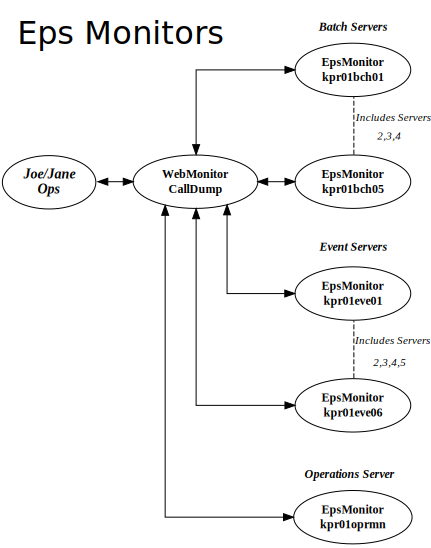
\includegraphics[width=10cm]{Pictures/EpsMonitors.png}
\end{document}
